\Chapter{REVUE DE LITTÉRATURE}\label{sec:RevLitt}




La recherche informatique appliquée à l'imagerie médicale se trouve à l'intersection de deux domaines et a par conséquent deux objets d'études: la conception d'algorithmes novateurs et la validation de ceux-ci suivant un protocole simulant un déploiement clinique. Les fondations de ce champs de recherche reposent donc à la fois sur des théories mathématiques statistiques et sur des considérations plus empiriques portant sur l'efficacité et l'utilisabilité des algorithmes dans un contexte clinique. Pour introduire notre recherche, on ne peut faire abstraction d'une description des emprunts faits à l'apprentissage machine et aux statistiques en général, emprunts réalisés non sans de nécessaires (et parfois substantielles) adaptations. \\
Afin de faciliter la compréhension du lecteur non initié, cette revue de littérature s'ouvre sur une introduction des principes théoriques constituant les briques fondamentales de la reconnaissance automatique d'images par apprentissage profond. Ainsi, les sections allant de \ref{sec:IntroductionVisionOrdinateur} à \ref{sec:interpretationProbabiliste} ont essentiellement une visée pédagogique. Les algorithmes qui y sont mentionnés appartiennent à la trousse à outils du chercheur, leur application n'est pas spécifique à un domaine en particulier. Nous y couvrons les opérateurs fondamentaux sur lesquels se basent les réseaux de neurones, un survol historique des architectures qui ont marqué ces dix dernières années (dont plusieurs réapparaîtront dans nos expériences) et un rappel sur les méthodes d'entraînement de celles-ci.
\\
À partir de la section \ref{sec:NoisyLabelLearning}, nous concentrons notre revue de littérature sur les éléments qui occupent le cœur de cette thèse: ainsi, dans la  section \ref{sec:theorieApprentissage}, nous introduirons le concept de généralisation et les éléments statistiques qui appartiennent à ce domaine. Cette présentation est découpée en une première introduction théorique suivie de considérations plus empiriques sur les questions d'adaptation de domaines et d'apprentissage sur cible bruitée. 
\\
La section \ref{sec:interprétabilitéModel} présente les notions d'explicabilité et d'interprétabilité des modèles, c'est-à-dire la compréhension qu'un utilisateur humain peut avoir de leur fonctionnement. Plus spécifiquement, nous nous concentrons sur le champs de recherche dédié aux méthodes de génération d'attribution locale.
\\
Enfin, à partir de la section \ref{sec:RevueLittOphtal}, nous aborderons plus spécifiquement les applications propres à l'ophtalmologie des modèles d'apprentissage machine, en discutant de la segmentation sémantique de lésions du \fundus{} et des approches locale et globale de classification par maladie.
\section{Réseaux de neurones dédiés à la vision par ordinateur}
\label{sec:IntroductionVisionOrdinateur}
\subsection{La trousse à outils numérique de l'apprentissage profond}

L'apprentissage machine est un champs englobant de nombreux concepts et algorithmes inventés au fil du développement de l'informatique. S'il ne fallait leur trouver qu'un seul point commun, ce serait de s'appuyer sur un ensemble de données observées pour construire une représentation statistique des relations qui régissent ces données. En cela, l'apprentissage machine se distingue des modélisations mathématiques ou physiques plus traditionnelles car il ne cherche pas à identifier explicitement les mécanismes de cause à effet; mais plutôt à dévoiler les corrélations statistiques qui expliquent au mieux les données observées. L'hypothèse qui prévaut est que si l'observation est suffisamment exhaustive, le modèle statistique s'approchera au plus près de la loi réelle qui régit le phénomène observé. \\
Dans ce vaste univers qu'est l'apprentissage machine, nous n'aborderons directement qu'une sous-catégorie, dite de l'apprentissage profond. Celle-ci a largement accaparé les devants de scènes scientifiques mais aussi médiatiques. Il faut noter que ses contours ne sont pas forcément unanimement définis, mais la grande majorité des travaux qui se revendique de l'apprentissage profond repose sur une forme plus ou moins évoluée de réseaux de neurones. 
Afin d'introduire ce domaine, nous souhaitons définir en premier lieu les grandes briques fonctionnelles utilisées par les réseaux de neurones. Les deux prochaines sous-sections sont donc à aborder comme une sorte de lexique simplifié; ce n'est qu'à partir de la section \ref{sec:ReseauxNeurones} que nous rentrerons dans les détails de la littérature sur le sujet.

\subsubsection{Le neurone formel}
Dans sa conception originale, le neurone formel s'inspire de son équivalent biologique: ce dernier possède plusieurs dendrites (modélisées comme des entrées) et un axone (modélisé comme une sortie). Les dendrites reçoivent un influx nerveux en provenance d'autres neurones (plus exactement de leur terminaison axonale) au niveau des synapses: ces influx sont modélisés sous forme de signaux numériques. L'opération réalisée par le neurone est modélisée comme une somme pondérée de ses entrées, puis, si cette somme franchit un certain seuil, sa transmission à sa sortie. Ainsi, dans sa forme la plus épurée, le neurone formel à $N$ entrées réalise simplement l'opération suivante:
\begin{equation}
	\label{eq:NeuroneFormel}
	y = \sigma(\sum_{i = 1}^N x_i w_i + b)
\end{equation}
où $\mathbf{x} \in \mathbb{R}^N$ est son entrée et $y \in \mathbb{R}$ sa sortie.
L'opérateur $\sigma$ représente une fonction de seuil, aussi dite d'activation. Elle est non-linéaire et distingue le neurone formel d'une simple projection linéaire. Les paramètres $\mathbf{w} \in \mathbb{R}^N$ et $b \in \mathbb{R}$ (appelés respectivement poids et biais) sont ses variables d'ajustemement qui, modifiées en fonction de l'objectif visé, permettent au neurone de produire la sortie attendue et donc \og d'apprendre \fg. L'équation \ref{eq:NeuroneFormel} peut se réécrire de manière équivalente sous sa forme vectorielle: $y = \mathbf{w}^T\mathbf{x} + b$. \\
En pratique, on n'utilise jamais un seul neurone isolé mais plutôt une couche de neurones (qui n'est rien d'autres que le calcul parallèle de $M$ neurones). Avec $\mathbf{x} \in \mathbb{R}^N$, $\mathbf{y} \in \mathbb{R}^M$, $\mathbf{b} \in \mathbb{R}^M$ et $\mathbf{W} \in \mathbb{R}^{N\times M}$, l'équation d'une couche neuronale s'obtient de manière similaire à celle de l'équation \ref{eq:NeuroneFormel}:
\begin{equation}
	\label{eq:CoucheNeuroneFormel}
	\mathbf{y} = \sigma(\mathbf{W}^T\mathbf{x} + \mathbf{b})
\end{equation}

Enfin, revenons sur la fonction d'activation $\sigma$: de nombreuses propositions existent dans la littérature, nous en recensons quelques unes sur la figure \ref{fig:activations_functions}. Elles modélisent en général un effet de saturation (limite finie vers $+/- \infty$), qui s'interprète comme un seuil au delà duquel le neurone s'active.
\begin{figure}[htb]
	\centering
	\includegraphics[width=\textwidth]{revue_litterature/activation_functions.png}
	\caption{Fonctions non-linéaires usuelles placées en sortie de neurones}
	\label{fig:activations_functions}
\end{figure}

\subsubsection{Le réseau de neurones multicouches}
En ayant introduit le neurone formel et son corollaire, la couche de neurones, nous disposons des bases nécessaires pour définir le premier réseau de neurones, dit multicouches. Son principe est simple: à l'instar du cerveau et son imbrication complexe de neurones, il est possible d'organiser un réseau artificiel sous la forme d'une succession de couches, connectées les unes aux autres de manière séquentielle. Autrement dit, la sortie de la couche $l$ est fournie en entrée de la couche $l+1$. Pour chacune, l'équation \ref{eq:CoucheNeuroneFormel} est respectée, même si chaque couche peut disposer d'une fonction d'activation qui lui est propre. Ce faisant, un réseau peut s'interpréter comme une composition (au sens mathématique) alternant projection linéaire et non-linéarité via la fonction d'activation:
\begin{equation}
	\mathbf{y} = \mathcal{F}(\mathbf{x}) = (\sigma^{(L)} \circ f^{(L)}) \circ ...\circ(\sigma^{(l)} \circ f^{(l)}) \circ ... \circ(\sigma^{(0)} \circ f^{(0)})(\mathbf{x}) 
\end{equation}
Sémantiquement, toutes les couches d'indice $l \in \left\lbrace 0, 1, ..., L-1\right\rbrace $ sont appelées couches cachées et leur nombre $L$ est référé sous le terme de profondeur du réseau. Par analogie, on parle de largeur pour désigner le nombre de neurones par couche. Ces deux paramètres (largeur et profondeur) font partie des choix architecturaux à faire dans la conception d'un modèle. Depuis les années 80, l'expressivité de $\mathcal{F}$ (c'est-à-dire sa capacité à approximer n'importe quelle fonction) est largement étudiée, dépendamment de la largeur et de la profondeur choisies. Les travaux de Cybenko G. sont précurseurs en la matière: il y introduit un des Théorèmes d'Approximation Universelle, démontrant la capacité d'un réseau de profondeur $d=1$ (une couche cachée) utilisant la fonction sigmoïde à approcher n'importe quelle fonction dès lors que sa largeur est assez grande (possiblement infinie). Des versions plus modernes de ces travaux généralisent ce théorème à différents types de non-linéarité. Depuis les travaux de travaux de Zhou et al. \cite{luExpressivePowerNeural2017} la tendance récente est à promouvoir une largeur bornée et une profondeur accrue. Cai et al. \cite{caiAchieveMinimumWidth2023a} explicitent, sous certaines conditions, une borne minimale à la largueur nécessaire.

\subsubsection{Quelques autres opérateurs usuels}
Dans la trousse à outils du concepteur de réseaux de neurones, d'autres opérateurs reviennent très fréquemment, sans que leur paternité ne soit très clairement définie: c'est en particulier le cas du \textit{Pooling} et du \textit{Softmax} \footnote{Nous conservons dans cette thèse les termes anglais à défaut d'une traduction adoptée unanimement par la communauté francophone}.

\paragraph{Le Pooling}est une opération de sous-échantillonnage très simple: au sein d'une fenêtre donnée, il s'agit d'aggréger la sortie de plusieurs neurones en une seule valeur. En pratique, on utilise fréquemment de deux types de pooling:
\begin{itemize}
	\item Le \textit{Max-Pooling} qui consiste à prendre la valeur maximale parmi les neurones dans la fenêtre considérée.
	\item Le \textit{Mean-Pooling} qui effectue la moyenne des neurones dans cette fenêtre.
\end{itemize}
Il n'existe pas nécessairement de justification théorique sur l'utilisation de l'une ou l'autre des méthodes; on peut simplement noter que le Max-Pooling est nettement prévalent.
\paragraph{Le Softmax} est une opération de normalisation $f: \mathbb{R}^d  \mapsto \left[0, 1 \right]^d$ définie par:
\begin{equation}
	f(\mathbf{x}) = \frac{\exp(\mathbf{x})}{\sum_i \exp(\mathbf{x}_i)}
\end{equation}
Généralement appliqué en sortie de la dernière couche d'un réseau de neurone, le Softmax ramène toutes les valeurs des neurones dans un intervalle fermé $\left[0, 1 \right]$. Par ailleurs, il contraint la somme de ces neurones à valoir 1. Pour cette raison, la sortie d'un softmax s'interprète généralement comme une distribution discrète de probabilités.


\subsection{Réseau de Neurones Convolutifs}
\label{sec:ReseauxNeurones}
La conceptualisation et l'étude de nouvelles architectures de réseau de neurones ont constitué une majeure partie des publications récentes (période 2012-2023). Comme le formulent Alzubaidi et al., cet aspect de la recherche représente le noyau dur de l'\textit{Apprentissage Profond} \cite{alzubaidiReviewDeepLearning2021}.
\\
Nous mettons ici l'accent sur les principales avancées obtenues en reconnaissance automatisée dans le domaine de la vision par ordinateur, donc sur des images. Dans ce domaine et bien avant l'émergence des réseaux neuronaux, l'opérateur de convolution est reconnu comme une clé de voûte de bien des algorithmes de traitement d'image. Connue pour ses propriétés dans le domaine du filtrage, la convolution est réinterprétée par Le Cun et al. \cite{lecunGradientbasedLearningApplied1998} qui proposent de rendre son noyau entraînable par descente de gradients. Cette idée, sans être conceptuellement révolutionnaire, a une grande importance théorique et pratique. La convolution n'étant qu'une projection linéaire locale, son interprétation sous le prisme de la théorie du neurone formel est assez directe. L'idée fondamentale des auteurs est remplacer les premières couches de neurones classiques par des couches convolutives, décomposant ainsi le réseau en une première partie liée à l'extraction de caractéristiques locales et une seconde à l'aggrégation et la classification de celles-ci.
L'architecture résultante, appelée LeNet-5, devient donc le premier \ac{CNN} (Figure \ref{fig:lenet}). Elle est composée de 4 couches convolutives suivies d'un \ac{PMC} à deux couches. Dans le détail, chaque couche convolutive est constituée d'un ensemble de filtres, dont les sorties sont concaténées pour former un tenseur de cartes de caractéristiques. Formellement, notons $f^k$ la fonction réalisée par la couche convolutive $k$. Celle-ci est paramétrée par un vecteur de poids $\mathbf{W}^k \in \mathbb{R}^{I \times O \times M \times N}$ et de biais $\mathbf{B} \in \mathbb{R}^I$. Les dimensions $M \times N$ représentent la taille du noyau de convolution. Cette fonction reçoit un tenseur d'entrée $\mathbf{X}^k \in \mathbb{R}^{I \times H \times W}$ et produit en sortie un tenseur $\mathbf{Y}^k \in \mathbb{R}^{O \times H' \times W'}$ 
\begin{equation}
	\mathbf{Y}^k = f^k(\mathbf{X^k})
\end{equation}
L'équation détaillée d'une couche convolutive est donnée par:
\begin{equation}
	\mathbf{Y}^k[o, h, w] = \sum_{i=1}^{I}\sum_{m, n=1}^{M, N}\mathbf{X}^k[i, h +m - \lfloor M/2 \rfloor, w +n - \lfloor N/2 \rfloor] \cdot \mathbf{W}^k[i, o, m, n] + \mathbf{B}[i]
\end{equation}

%\begin{figure}[htb]
%	\centering
%	\includegraphics[width=5in]{placeholder}
%	\caption{Description d'une opération de convolution au sein d'une couche convolutive}
%	\label{fig:convolution}
%\end{figure}

\begin{figure}
	\centering
	\includegraphics[width=0.7\textwidth]{gnuplot/revue_litterature/LeNet}
	\caption{Représentation simplifiée du réseau LeNet-4}
	\label{fig:lenet}
\end{figure}


La première dimension $I$ correspond aux canaux du tenseur d'entrée. Ainsi, $\mathbf{X}^0$ qui correspond à l'image d'entrée du réseau, possède généralement un ou trois canaux (monochrome, \og rouge, vert, bleu\fg) et $I \in \{ 1, 3\}$.  
Plusieurs propriétés se dégagent de cette définition de convolution neurale:
\begin{itemize}
	\item Si $\mathbf{W}$ est symétrique, l'opération de convolution décrite correspond à la définition de la corrélation au sens du traitement du signal.
	
	\item $f^k$ est linéaire. En conséquence, $f^{k'} \circ f^{k}$ est également linéaire; par extension, un réseau constitué d'une succession de couches convolutives ainsi définies se réduirait à une application linéaire; ce qui n'est pas souhaitable pour l'expressivité de l'architecture globale. Pour cette raison, on introduit une non-linéarité en sortie de chaque couche convolutive, à l'instar du neurone formel standard.

	\item La taille du masque de convolution $M \times N$ correspond à la notion de champs de vision de la couche, autrement dit du nombre de points de l'image d'entrée considéré pour le calcul de la sortie. En conséquence, la taille du masque est indicatrice du contexte spatial que la couche convolutive est en mesure de prendre en compte dans son calcul de sortie.
	
	\item L'opération de convolution est équivariante en translation, ce qui revient à dire que la même projection linéaire appliquée localement se fait sur toute l'image.
\end{itemize}

 Dans la grande majorité des cas, les architectures se composent en successions séquentielles de couches de convolutions, réduisant progressivement la résolution spatiale des cartes de caractéristiques tout en accroissant la largeur de chaque couche (le nombre de cartes extraites). De la sorte, le réseau effectue une agrégation spatiale de l'information contenue dans l'image, tout en allouant une dimension croissante au vecteur caractéristique assigné à chaque position spatiale, permettant à cette agrégation de gagner en abstraction (c'est-à-dire en capacité à représenter des structures de plus en plus complexes et spatialement éloignées dans l'image). 
 Dans les dernières couches, la résolution de l'image d'entrée se retrouve suffisamment réduite pour qu'elle puisse facilement se représenter sous la forme d'un vecteur, qu'il est possible de classifier via une succession de couches de neurones totalement connectés. L'intérêt de l'approche est d'automatiser entièrement l'étape de d'extraction et de sélection de caractéristiques, la partie convolutive du réseau étant entraînée à la faire conjointement à la classification. Comme nous le verrons, l'apprentissage présente l'avantage théorique de garantir l'extraction de caractéristiques localement optimales.

Khan et al. \cite{khanSurveyRecentArchitectures2020} proposent une revue de littérature détaillée des avancées techniques et conceptuelles dans le domaine des \ac{CNN}s au cours  de la dernière décennie. Nous en dressons ici une synthèse présentant les grandes architectures représentant des jalons importants dans l'histoire des réseaux de neurones. Au delà du seul intérêt historique, cette présentation introduit les éléments architecturaux utilisés par nos propres modèles. La modularité est en effet une notion fondamentale pour comprendre le succès des réseaux de neurones modernes.

\paragraph{AlexNet}
Proposée par Krizhevsky et al. \cite{krizhevskyImageNetClassificationDeep2012}, AlexNet (du nom de son auteur) est l'une des plus emblématiques architectures de \ac{CNN}. Quinze ans après les travaux précurseurs de Le Cun et al. \cite{lecunGradientbasedLearningApplied1998}, AlexNet surpasse spectaculairement l'état de l'art dans la classification de large base de données d'images (en l'occurance la version de 2010 du \ac{ILSVRC} \cite{dengImageNetLargescaleHierarchical2009}, constituée de 1.4 millions d'images réparties en 1000 classes). Outre une optimisation des calculs par parallélisation sur \ac{GPU}, AlexNet présente trois évolutions notables (par ailleurs également introduites en collaboration avec Hinton et al. \cite{hintonImprovingNeuralNetworks2012}):
\begin{itemize}
	\item L'utilisation d'une normalisation de la réponse locale en sortie de certaines couches.
	\item La régularisation du modèle pour éviter le sur-apprentissage par utilisation de la technique du \textit{Dropout}, c'est-à-dire la mise à zéro aléatoire de certains neurones. 
	\item L'utilisation de la fonction \ac{RELU} en sortie des couches convolutives (voir Figure \ref{fig:activations_functions})
\end{itemize}
Ce modèle marque le début du regain d'intérêt pour les \ac{CNN}s et une prise en compte de l'intérêt des \ac{GPU} pour les calculs hautement parallélisables (et autres que les opérations graphiques qui leur étaient réservées). En 2007, NVIDIA, fabriquant leader sur le marché des \ac{GPU}s met à disposition \ac{CUDA}, une librairie proposant une extension du langage C pour le calcul parallèle sur \ac{GPU}. En 2014, prenant la mesure de l'importance que prennent les réseaux de neurones, l'entreprise sort \textit{cuDNN}, une librairie additionnelle offrant un ensemble d'implémentations pré-écrites pour les opérations usuelles qu'utilisent ces algorithmes.

\paragraph{VGG}
\label{par:VGG}
L'architecture VGG (du nom du laboratoire dont elle est issue, le \textit{Visual Geometry Group}) \cite{simonyanVeryDeepConvolutional2015a} est également considérée comme une étape majeure dans l'évolution des \ac{CNN}s. Structurellement, il s'agit toujours une succession de couches convolutives; mais le VGG accumule en davantage, accroissant ainsi la profondeur du réseau. Pour y arriver, Simonyan et al. proposent de remplacer les masques de convolutions du AlexNet (originellement de taille $7 \times 7$ ou $5 \times 5$ ) par des masques plus petits ($3 \times 3$ voire $1 \times 1$). Le nombre de paramètres entraînés étant égal au carré de la taille du masque, réduire cette dernière permet d'augmenter le nombre de couches. Le réseau gagne ainsi en profondeur. Cependant, un masque de taille $5 \times 5$ a un champs visuel réceptif naturellement plus élevé qu'un masque plus petit, ce qui peut sembler un argument important en faveur des masques de grande taille. Simonyan et al. le contrent en arguant que le champs réceptif s'accroit linéairement à chaque couche convolutive. Suivant cette logique, il est possible d'obtenir un champs réceptif de taille $5 \times 5$ en utilisant deux couches de taille $3 \times 3$ successives (la figure \ref{fig:TheoricalReceptiveField} illustre ce phénomène): ce faisant, par rapport à un seul masque de $5 \times 5$, on réalise une économie de $5 \times 5 - (2\cdot (3\times 3)) = 7$ paramètres (soit 28\% de moins). De plus, à chaque opération de sous-échantillonnage insérée entre deux couches (on parle de \textit{pooling}), le champs réceptif visuel théorique est doublé.

\begin{figure}[htb]
	\centering
	\includegraphics[width=0.5\textwidth]{revue_litterature/3by3equal5.png}
	\caption{Illustration de la notion de champs visuel réceptif obtenu par la mise en séquence de deux couches convolutives de masque $3 \times 3$. Pour obtenir la valeur du pixel rouge, il faut prendre les $3 \times 3$ pixels de l'image de la couche précédente, eux-même tous obtenus en utilisant les $5\times 5$ pixels de la couche d'entrée. On peut donc parler de champs visuel réceptif de $5 \times 5$ pour la troisième couche.}
	\label{fig:TheoricalReceptiveField}
\end{figure}
Notons cependant que la notion de champs visuel théorique ne correspond pas à une réelle mesure d'importance d'un pixel d'entrée de réseau vis-à-vis d'un pixel en sortie d'une des couches convolutives. Il s'agit plutôt d'une borne supérieure, en pratique jamais atteinte, sur le contexte spatial pris en compte dans l'estimation de la sortie d'une couche donnée. Luo et al. proposent une estimation probabiliste du champs visuel réceptif effectif \cite{luoUnderstandingEffectiveReceptive2016} faisant l'hypothèse d'une distribution Gaussienne des noyaux des masques convolutifs. Ils démontrent que le champs visuel réceptif effectif est en pratique bien inférieur à son estimation théorique.

\paragraph{Inception-V1}
Contemporain du VGG, Szegedy et al. proposent le GoogleNet, s'appuyant sur un nouveau type de module appelé \textit{Inception-block} \cite{szegedyGoingDeeperConvolutions2015a}. Les auteurs documentent également l'utilisation d'un certain nombre de techniques permettant de réduire le nombre de paramètres du réseau par couches (et donc d'augmenter le nombre de celles-ci). En particulier, leur architecture fait usage de convolution de taille $1 \times 1$. En apparence, une telle opération n'est qu'une combinaison linéaire des cartes de caractéristiques qui lui sont fournies. Elle permet cependant d'en réduire la dimension, à l'instar d'un opérateur de compression. De plus, l'ajout d'une fonction non-linéaire à la sortie de chacune des convolutions $1 \times 1$ permet la composition de fonctions de plus en plus complexes.
Quant à lui, le bloc \textit{Inception} (Figure \ref{fig:InceptionBlock}) a pour principale originalité la mise en parallèle de diverses couches convolutives, chacune ayant sa propre paramétrisation (différentes tailles de masque). Les caractéristiques extraites par chaque couche sont ensuite fusionnées via un opérateur dédié.

\begin{figure}[htb]
	\centering
	\includegraphics[width=.4\textwidth]{revue_litterature/module_inception}
	\caption{Illustration de l'\textit{Inception block} proposé par Szegedy et al. pour l'architecture GoogleNet \cite{szegedyGoingDeeperConvolutions2015a}}
	\label{fig:InceptionBlock}
\end{figure}

L'utilisation de ces voies parallèles oriente la recherche vers des réseaux de plus en plus profonds, c'est-à-dire constituée de séquences de couches toujours plus longues. Or, deux problèmes sont rapidement identifiés:
\begin{itemize}
	\item La composition de fonctions entraîne une évanescence (ou au contraire, une explosion) des gradients sur certaine couche lors de l'opération de rétro-propagation. Dans une certaine mesure, cet effet peut être contrôlé par une initialisation judicieuse des poids du modèle\cite{glorotUnderstandingDifficultyTraining2010, heDelvingDeepRectifiers2015} ou l'utilisation de couches de normalisations intermédiaires \cite{ioffeBatchNormalizationAccelerating2015, ulyanovInstanceNormalizationMissing2016a, baLayerNormalization2016}.
	\item Il a été observé qu'un réseau plus profond est sujet à une dégradation de ses performances \cite{heConvolutionalNeuralNetworks2015a, srivastavaHighwayNetworks2015}, non seulement sur l'ensemble de test, mais également sur celui d'apprentissage. Un tel effet est contre-intuitif: ajouter des poids ne devrait théoriquement pas dégrader les performances sur l'ensemble d'apprentissage. En effet, dans le pire des cas, le réseau pourrait se passer des couches supplémentaires en les mappant vers la fonction identité. Cette dégradation n'est donc pas la conséquence d'un sur-apprentissage lié à un excès de paramètres.
\end{itemize}
Ces observations ont motivé la recherche vers de nouvelles formes d'architectures telles les \textit{Highway Network} \cite{srivastavaHighwayNetworks2015} ou les \textit{Residual Network} \cite{heDeepResidualLearning2016b}. Toutes deux ont pour objectif d'accroître la profondeur du réseau (jusqu´à plus de cent couches convolutives) tout en résolvant les problèmes liés aux gradients. Nous détaillons ici la dernière; ses performances l'ayant rendu très populaire, la rendant aujourd'hui encore très utilisée.

\paragraph{Residual Network}
\label{sec:resnet}
He et al. introduisent la notion de connexions résiduelles pour augmenter significativement le nombre de couches du réseau \cite{heDeepResidualLearning2016b}. Le raisonnement des auteurs est le suivant: si un ensemble de couches non linéaires successives peut approximer n'importe quelle fonction $\mathcal{H}(x)$, il lui est tout autant possible d'approximer la fonction résiduelle $\mathcal{F}(x) = \mathcal{H}(x) - x$. La fonction originale se retrouve donc simplement par addition $\mathcal{F}(x) + x$, qui est au c\oe ur du \textit{ResNet}: l'entrée d'une (ou plusieurs) couche est additionnée à sa sortie, on parle alors de connexion résiduelle. Cette \og astuce \fg permet d'accroître la taille du réseau: en effet cette connexion facilite la propagation des gradients. Par ailleurs, toute section $\mathcal{F}(x)$ du réseau potentiellement inutile pourra converger vers la fonction nulle; la connexion résiduelle assurant que l'identité sera conservée. Les auteurs démontrent que ces connexions améliorent grandement les performances d'un réseau profond (jusqu'à 101 couches), tout en maintenant celle d'un réseau plus superficiel.

\begin{figure}[htb]
	\centering
	\includegraphics[width=.7\textwidth]{revue_litterature/residual_connection}
	\caption{Connexion résiduelle proposée par He et al. pour l'architecture ResNet \cite{heDeepResidualLearning2016b}. Les convolutions $1\times 1$ placées en entrée et sortie sont optionnelles: elles permettent la projection des cartes de caractéristiques vers des espaces aux dimensions concordantes si nécessaire.}
	\label{fig:ResNet}
\end{figure}

\paragraph{DenseNet}
Huang et al. étendent le concept des connexions résiduelles à travers une nouvelle architecture nommée DenseNet \cite{huangDenselyConnectedConvolutional2017}. À l'inverse du ResNet, pour lequel les connexions résiduelles sont arbitrairement choisies, le DenseNet s'appuie sur un principe de connexion complète: chaque sortie de couche est envoyée en entrée de toutes les couches suivantes appartenant a un même bloc, où chaque bloc est délimité par une opération de pooling. Autrement dit, toutes les couches au sein d'un même bloc possède la même résolution spatiale. Au sein d'un bloc de $L$ couches, il existera donc $\frac{L\cdot(L+1)}{2}$ connexions au lieu des $L+1$ du ResNet. Autre différence avec ce dernier, la connexion résiduelle ne se fait pas par une addition, mais avec une concaténation des cartes de caractéristiques. Pour limiter une sur-paramétrisation du modèle, chaque couche est limitée à douze cartes de sortie, ce qui est significativement plus petit que dans les précédents travaux décrits. Malgré cela, les auteurs obtiennent des performances supérieures à l'état de l'art et montrent que grâce à ces connexions \og denses\fg, le problème des gradients évanescents disparaît. Une des hypothèses fournies pour expliquer cette efficacité repose sur l'idée que la structure dense favorise la réutilisation des caractéristiques entre couches successives, ce qui va dans le sens d'un meilleur signal propagé.

\paragraph{SqueezeNet}
\label{par:squeezeNet}
Inspirés par les premiers modèles d'attention (\cite{wangResidualAttentionNetwork2017}), Hu et al. \cite{huSqueezeandExcitationNetworks2018} proposent une nouvelle architecture appelée SqueezeNet. Son originalité repose sur le module \textit{Squeeze-\&-Excite}. L'idée, là encore, est d'élargir le contexte spatial pris en compte dans une couche convolutive: en effet, le noyau de convolution basique n'a un effet que local, les relations contextuelles à plus large échelle sont donc ignorées. Jusqu'ici, cet effet a été corrigé en accumulant séquentiellement les couches convolutives, mais Hu et al. proposent une autre approche. L'idée est de construire, pour chaque couche, un vecteur contextuel encapsulant les relations globales. Celui-ci est obtenu par \textit{Global Mean Pooling} (c'est-à-dire la moyenne spatiale du tenseur des caractéristiques en sortie de couches), avant d'être fourni à un simple réseau \ac{PMC} à deux couches qui maintient les dimensions du vecteur. La première étape correspond au compression des caractéristiques (\textit{Squeeze}), la seconde à leur excitation. Le vecteur résultant est ensuite passé à travers une fonction sigmoïde $\sigma$ afin de borner ses valeurs dans l'intervalle $\left[ 0, 1\right]$. L'étape d'excitation consiste à multiplier ce vecteur au tenseur d'entrée, venant ainsi pondérer chacune des caractéristiques de celui-ci. Cette pondération est souvent associée à la notion d'attention, car elle permet de concentrer le réseau sur certaines cartes de caractéristiques précises. 

\subsection{Modèles de segmentation sémantique}
\label{sec:ModeleSegmentation}
Les modèles présentés dans la section précédente ont pour point commun de se limiter à la classification d'images. Autrement dit, pour une image, la sortie de ces réseaux aura la forme d'un vecteur indicateur de la classe prédite. Mais pour de nombreuses applications et tout particulièrement dans le domaine médical, il est souvent nécessaire d'obtenir une granularité plus fine et obtenir une classification à l'échelle du pixel plutôt que de l'image. Cette opération est appelée \textbf{segmentation sémantique}. Si les architectures présentées jusqu'ici ne sont pas initialement conçues pour cela, il est aisé de les adapter. Une façon de le faire est d'entraîner le modèle à prédire la classe d'appartenance d'un \textit{patch} (morceau) d'image; en recombinant chaque patch, on reconstruit une image segmentée. On retrouve dans l'idée cette approche dans les travaux précurseurs de Farabet et al. \cite{farabetLearningHierarchicalFeatures2013}. L'inconvénient de cette approche est de limiter la prise en compte du contexte à la taille du patch considéré. Farabet et al. résolvent ce problème par l'utilisation des \ac{CRF}, méthode qui suit la théorie statistique des Champs de Markov et qui regroupe les pixels présentant une apparence similaire à travers l'image conditionnellement à une pré-segmentation. Il s'agit donc d'une étape de post-traitement qui a pour avantage de prendre en compte le contexte global de l'image. Le second inconvénient du modèle de Farabet et al. est de produire une  segmentation dont la résolution est tributaire de la taille du patch choisi: plus celui-ci est grand, plus la résolution sera faible. Mais inversement, pour des petits patches, segmenter toute l'image prendra un temps considérablement plus long. \\
Ces deux inconvénients ont poussé au développement d'un nouveau type d'architecture de réseau de neurones que nous présentons ici.
\subsubsection{Réseau entièrement convolutif}
\label{sec:FCCN}


Long et al. \cite{longFullyConvolutionalNetworks2015a} seront les premiers à se passer d'une couche de classification dans leurs travaux sur la segmentation. Plutôt que de reprendre la structure conventionnelle: $N \times (\text{Couches convolutives} \rightarrow \text{Pooling}) \rightarrow K \times \text{Couches totalement connectées} \rightarrow \text{Classification}$ (qui décrit plus ou moins toutes les architectures de la section précédente), les auteurs suggèrent de ne garder que la première étape (les $N$ couches convolutives), afin de conserver la structure spatiale des cartes de caractéristiques que le pooling détruit. Chacun des pixels appartenant à ces cartes est ensuite projeté vers sa classe prédite. Ce faisant, au lieu de passer d'une fonction de coût par image, on obtient une fonction de coût par pixels. La spécificité de cette architecture est donc de n'utiliser que des couches convolutives et de ré-échantillonnage (pooling, unpooling ou interpolation). En revanche, dans les travaux de Long et al. la prédiction finale reste raffinée par l'utilisation des \ac{CRF}. L'opération de ré-échantillonnage permet d'interpoler les cartes de caractéristiques vers la résolution initiale de l'image d'entrée. Cette opération peut se faire aussi bien par simple interpolation bilinéaire que par déconvolution.
\paragraph{DeepLab-V3}
L'architecture DeepLab-V3, introduite en 2017 par Chen et al. \cite{chenRethinkingAtrousConvolution2017} franchit un palier technologique, en obtenant de hautes performances malgré l'absence d'utilisation d'un post-traitement de type \ac{CRF}. Comme son nom l'indique, il s'agit de la troisième itération d'une architecture dont chaque composant a été soigneusement testé. Elle se caractérise par l'utilisation de blocs basés sur l'idée des connexions résiduelles de type ResNet (paragraphe \ref{sec:resnet}) et surtout l'introduction du module ASPP (pour \textit{Atrous Spatial Pyramid Pooling}). La notion de convolutions atrous (à trous) est fondamentale pour cette architecture, en cela qu'elle permet, à moindre frais, la prise en compte d'un plus grand contexte spatial et sans ajouter de paramètres au modèle. Son mécanisme est illustré sur la figure \ref{fig:aTrousConvolutions}.

\begin{figure}[!h]
	\centering
	\begin{subfigure}[t]{0.48\textwidth}
	\includegraphics[width=\textwidth]{revue_litterature/convolutions_a_trous.png}
	\caption{Principe illustrée de la convolution à trous (ou dilatées). Pour un même nombre de paramètres (ici $3 \times 3$), le champs réceptif est artificiellement accru en les espaçant.}
	\end{subfigure}
	\hfill
	\begin{subfigure}[!ht]{0.45\textwidth}
		\includegraphics[width=\textwidth]{revue_litterature/ASPP}
		\caption{Module ASPP. La variable $d$ indique les différents coefficients de dilatation.}
	\end{subfigure}

	\caption{Illustrations des modules utilisées dans l'architecture DeepLabV3\cite{chenRethinkingAtrousConvolution2017}}
	\label{fig:aTrousConvolutions}
\end{figure}

\paragraph{U-Net}
\label{par:Unet}

Introduite par Ronneberger et al. \cite{ronnebergerUNetConvolutionalNetworks2015b}, l'architecture U-Net est certainement une des plus emblématiques en ce qui concerne la segmentation sémantique d'image médicale, du moins la plus citée. Outre sa simplicité, un de ses plus gros atouts est sa capacité à générer d'excellentes performances même en disposant que de peu de données d'entraînement. Une représentation de l'architecture est fournie sur la figure \ref{fig:UnetArchitecture}. Sa structure respecte le principe, souvent repris depuis, d'encodeur/décodeur. L'encodeur fonctionne similairement à la plupart des architectures présentées jusqu'ici, c'est-à-dire en compressant progressivement les dimensions spatiales de l'image tout en enrichissant le vecteur descriptif à chaque pixel de nouvelles composantes. Le décodeur pour sa part fait l'exact inverse et ré-interpole progressivement les cartes de caractéristiques jusqu'à la dimension de l'image. Cependant, le U-Net se distingue de ce simple principe en ajoutant des connexions passerelles entre chaque étape de l'encodeur et du décodeur. Celles-ci ont deux objectifs:
\begin{itemize}
	\item Maintenir la propagation des gradients intacte malgré le nombre de couches du réseau, similairement à ce que fait le ResNet.
	\item Affiner les détails de segmentation des petites structures. En effet, du fait du principe de sous-échantillonnage/ré-interpolation, les réseaux de segmentation ont tendance à effacer les plus petites structures. En ajoutant ces connexions passerelles, le U-Net corrige cet effet.
\end{itemize}
\begin{figure}[!htb]
	\centering
	\includegraphics[width=.7\textwidth]{revue_litterature/unet}
	\caption{Architecture originale du U-Net}
	\label{fig:UnetArchitecture}
\end{figure}
\paragraph{Variantes du U-Net}
L'architecture du U-Net est fondatrice pour sa structure en \og U\fg basé sur un couple encodeur/décodeur symétrique. Peut-être en raison de sa facilité d'implémentation, ce concept a inspiré une pléthore de variantes. Bien souvent, les améliorations proposées s'appuient sur des modules empruntés à d'autres architectures pré-existantes. Par exemple, Rundo et al. \cite{rundoUSENetIncorporatingSqueezeandExcitation2019} créent le SE-U-Net en incorporant le module Squeeze-\&-Excite dans les différentes couches d'encodeur et décodeur pour la segmentation d'image d'IRM, Oktay et al. \cite{oktayAttentionUNetLearning2022} ajoutent un mécanisme d'attention sur une variante du U-Net adaptée aux images tridimensionnelles dédiée à la segmentation du pancréas, Zhou et al. \cite{zhouUNetRedesigningSkip2020} étendent le concept des connexions denses (de type \textit{DenseNet}) entre les couches d'encodage et décodage de leur réseau appelé U-Net++. 
\\
Il ne s'agit là que de quelques exemples parmi de nombreux autres, qui témoignent parfaitement de la modularité des architectures de réseaux de neurones. 

\newpage

\subsection{Optimisation et entraînement de modèles}
Malgré la diversité des architectures, il est remarquable que celles-ci adoptent essentiellement la même stratégie pour ajuster leurs paramètres lors de la phase d'entraînement. Cette section a pour objectif de clarifier ce mécanisme de manière formelle pour s'accorder sur une définition de l'apprentissage. Précisons que nous nous limitons ici au problème de l'apprentissage supervisé (autrement dit, pour lequel il existe une référence explicite à atteindre, appelée vérité terrain). Bien souvent le cas de l'apprentissage non-supervisé aborde l'entraînement de manière similaire, avec cependant une reformulation de l'objectif visé. \\
Dans un cas comme dans l'autre, l'entraînement utilise un jeu de données, en pratique souvent de taille conséquente, pour mettre à jour les paramètres du modèle de manière itérative. Ce processus s'arrête une fois la convergence atteinte vers un modèle jugé satisfaisant. Nous le détaillons ici.\\

Soit un jeu de données $\mathcal{S} = \{ (x_m, y_m) \in \mathbb{R}^d \times \{1, ...,K\}^{d'}\}, |S|=M$, c'est à dire $M$ échantillons ($x_m$ de dimension $d$), chacun venant avec une classe associée représentée par le label $y_m$ prenant valeur parmi les $K$ classes possibles. La dimension $d'$ du vecteur de label dépend de l'application considérée: ainsi pour la classification d'images, en général $d'=1$ (une seule classe par image), pour la segmentation sémantique, $d'=d=H\times W$ où $H, W$ représentent la hauteur et la largeur de l'image (une classe par pixel de l'image). \\
Le réseau de neurones que l'on souhaite entraîner est représenté sous la forme d'une fonction $f_\theta: \mathbb{R}^d \to  \{1, ...,K\}^{d'}$, où $\theta$ englobe tous les paramètres (ou poids) du modèle. 
Cette configuration représente le cas typique rencontré pour l'apprentissage supervisé d'un modèle multiclasse (y compris pour de la segmentation).
Un modèle $f_{\theta^\star}$ idéalement entraîné sur les données $\mathcal{S}$ saura faire une association parfaite entre $x_m$ et sa classe associée par la vérité terrain\footnote{Il s'agit d'une simplification volontaire, car la sortie d'un réseau de neurones est continue et non discrète. En réalité, on modélise plutôt la sortie réseau comme une estimation de la probabilité d'appartenance à chaque classe.}, c'est-à-dire : 
\begin{equation}
	f_{\theta^\star}(x_m) = y_m, \forall\, 1 \leq m \leq M
\end{equation} 
En revanche, un modèle non-idéal commettra des erreurs. On les quantifie par une fonction de coût (ou d'erreur) notée $\mathcal{L}(f_\theta(x_m), y_m)$ évaluée pour chaque point de $\mathcal{S}$. En la calculant sur l'ensemble des données, on obtient une fonction de coût global:
\begin{equation}
	J(\theta) = \sum_{m=1}^{M} \mathcal{L}(f_\theta(x_m), y_m)
\end{equation}
Seule la dépendance à $\theta$ est indiquée dans la fonction d'erreur $J$, car il s'agit de la seule variable d'intérêt à optimiser. 
À titre d'exemple, la fonction d'erreur au carré moyenne (connue sous le nom de \ac{MSE}) mesure directement l'écart entre la sortie du modèle et le label associé à son entrée\footnote{Le carré garantit la positivité de la fonction}:
\begin{equation}
	J(\theta) = \frac{1}{M}\sum_{m=1}^{M}(f_\theta(x_m) - y_m)^2
\end{equation}
En construisant ainsi une fonction de coût, on peut définir la notion d'entraînement de manière formelle: il s'agit de trouver les paramètres $\theta^\star$ qui minimiseront $J(\theta)$, c'est à dire qui diminueront l'erreur globale sur l'ensemble des données à disposition:
\begin{equation}
	\theta^\star = \argmin_{\theta} J(\theta)
\end{equation}
Le problème de cette minimisation se ramène à un calcul d'optimisation numérique que nous détaillons au prochain paragraphe. Mais ouvrons une courte parenthèse pour préciser qu'il s'agit d'une vision tronquée de l'apprentissage machine, qui en réalité s'appuie sur la théorie de l'apprentissage statistique et justifie l'entraînement d'un réseau comme une tentative de modélisation de la distribution de probabilités décrivant $\mathcal{S}$.
Cette interprétation probabiliste sera détaillée à la fin de cette section, mais nous fermons pour l'instant cette parenthèse pour revenir à la notion d'optimisation.
\subsubsection{Descente de gradients}
Abstraction faite de la théorie justifiant cette approche, l'entraînement d'un réseau de neurones se résume à un problème d'optimisation numérique d'une fonction d'erreur. Deux types de solutions existent pour un tel problème:
\begin{enumerate}
	\item Une solution unique $\theta^\star$ telle que $J(\theta^\star) \leq J(\theta), \forall \theta$ est qualifiée de minimum global.
	\item Si la solution identifiée n'est valable que dans un voisinage $\mathcal{N}$ de $\theta^\star$, c'est à dire $J(\theta^\star) \leq J(\theta), \forall \theta \in \mathcal{N}$, on parle alors de minimum local.
\end{enumerate}
Notons que si la fonction à optimiser $J$ est convexe, les minimum local et global se confondent. Une grande partie de la recherche en optimisation se concentre donc sur les problèmes convexes; mais il est bien connu que les réseaux de neurones n'appartiennent pas à cette catégorie.
Idéalement, l'entraînement devrait aboutir à une solution $\theta^\star$ globale: elle indiquerait ainsi la meilleure configuration de paramètres du modèle parmi l'ensemble des possibilités. En pratique, il est quasiment impossible d'identifier un minimum global et on se contente d'en rechercher un local (il peut y en avoir naturellement plus d'un). Il est aisé de reconnaître un minimum local en faisant quelques hypothèses faibles: il est nécessaire que la fonction de coût global, $J(\theta): \mathbb{R}^N \to \mathbb{R}$ soit différentiable presque partout (où $N$ est le nombre de paramètres du modèle). Tout minimum, local ou global, vérifie alors:
\begin{equation}
	\label{eq:OptimalPointTheta}
	\nabla J(\theta^\star) = 0
\end{equation}
La démonstration de ce résultat est une application quasi-directe du théorème de Taylor. L'équation \ref{eq:OptimalPointTheta} permet de définir un critère d'arrêt de l'entraînement, correspondant à la découverte d'un minimum local. Partant d'une initialisation $\theta_0$ du modèle, il reste alors à trouver le chemin menant à $\theta^\star$ (ou du moins une valeur approchée). Pour y arriver, tous les algorithmes d'optimisation génèrent une séquence $\{\theta_k\}_{k=0}^{\infty}$ et définissent des règles d'évolution. Il existe deux grandes stratégies pour trouver ces itérations. La première a trait à la recherche de ligne directrice (direction à prendre dans l'évalution des $\theta_k$) tandis que la seconde transforme le problème en la recherche d'une région de confiance (dans l'espace des paramètres); toutes deux ont fait l'objet d'importantes recherches ces cinquante dernières années largement documentées par Nocedal J. et Wright S. \cite{nocedalIntroduction2006}. 
\\
L'entraînement d'un réseau de neurone appartient à la première catégorie. À chaque itération $k$, la fonction de coût est évaluée au point $\theta_k$. On choisit ensuite une direction $p_k \in \mathbb{R}^N$ qui permet de décroître la fonction de coût et on se déplace le long de celle-ci sur une certaine longueur $\alpha_k \in \mathbb{R}^+$ avec pour objectif de remplir ces deux conditions:
\begin{equation}
	 \left\{ \begin{array}{cl}
		\theta_{k+1} &= \theta_k + \alpha_k p_k \\
		J(\theta_{k+1}) &\leq J(\theta_{k})
	\end{array} \right.
\end{equation}
Dans le contexte de l'entraînement d'un réseau de neurones, le scalaire $\alpha_k$ porte le nom de \textit{pas d'apprentissage}. 
\\
Toujours en s'appuyant sur la décomposition de Taylor de la fonction de coût, on peut montrer que la direction de plus forte diminution suit le gradient au point $\theta_{k}$. Dans le cadre de l'entraînement, on choisit donc généralement:
\begin{equation}
	p_k = -\nabla J(\theta_k)
\end{equation}
d'où l'appellation \og descente de gradients\fg tire son nom. Notons qu'il ne s'agit pas forcément de la direction optimale pour atteindre le minimum; uniquement la direction de plus forte descente au point considéré. La méthode de Newton suggère par exemple de calculer la direction:
\begin{equation}
	p_k = - \nabla^2 J_k ^{-1} \nabla J_k
\end{equation}
Qui fait intervenir la Hessienne inversée de la fonction $J$ au point $\theta_{k}$. Malheureusement, ni le calcul de dérivées d'ordre supérieur à 1 (pour la Hessienne), ni le calcul de son inverse ne sont en pratique réalisables pour un réseau de neurones. En effet, rappelons que $J$ a pour support $\mathbb{R}^N$, où $N$ représente le nombre de paramètres du modèle. Celui-ci peut se compter en milliers (voire bien plus pour les plus gros modèles). Cette complexité rend inutilisable une grande partie des techniques développées en optimisation numérique dès lors qu'il s'agit d'une architecture un tant soit peu conséquente.
De la même manière, il existe une abondante littérature sur le choix optimal du pas d'apprentissage en fonction de la direction choisie \cite{nocedalLineSearchMethods2006}, mais en pratique, l'entraînement d'un réseau de neurones utilise des heuristiques bien plus simples.

\subsubsection{Descente de gradients stochastique}
En choisissant $p_k = -\nabla J(\theta_k)$, l'algorithme de descente de gradients peut se réécrire:
\begin{align}
	\theta_{k+1} &= \theta_{k} - \alpha_k \nabla J(\theta_k) \\
	&= \theta_{k} - \alpha_k \nabla \sum_{m=1}^{M} \mathcal{L}(f_{\theta_k}(x_m), y_m)
\end{align}
Sous cette forme, il apparaît clairement que le calcul de l'estimateur $J(\theta_k)$ fait intervenir l'ensemble des données pour le calcul des contributions individuelles $\mathcal{L}$, et ce pour chaque itération $k$ d'apprentissage. Dans la pratique, où les données $\mathcal{S}$ peuvent contenir plusieurs milliers ou millions de points, il est bien souvent très inefficace (voire impossible) de calculer le gradient global. On peut en revanche en calculer une estimation. Pour cela, on définit la famille de parties $\{\mathcal{B}_i \subset \mathcal{S} | \bigcup_i \mathcal{B}_i = \mathcal{S} \} $ de telle sorte que chaque élément de $\mathcal{B}_i$ est tiré sans remise aléatoirement de $\mathcal{S}$. L'algorithme se base ainsi sur une estimation du gradient global sur un sous-ensemble de données:
\begin{equation}
	\theta_{k+1} = \theta_{k} - \alpha_k \nabla \sum_{m \in \mathcal{B}_i}\mathcal{L}(f_{\theta_k}(x_m), y_m)
\end{equation} 
À chaque itération $k$, un nouveau sous-ensemble $\mathcal{B}_i$ \footnote{Appelé \textit{mini-batch} en anglais} est choisi, correspondant donc à un échantillonnage aléatoire des données d'entraînement. On parle donc de descente de gradients stochastiques. Dépendamment d'hypothèses plus ou moins fortes, il est possible de démontrer la convergence uniforme d'un tel processus itératif. Mais nous nous contenterons ici de cette description sommaire, suffisante pour introduire une technique qui appartient en réalité au vaste domaine des algorithmes stochastiques et des martingales, pour lequel il existe de nombreux résultats théoriques fondamentaux \cite{godichon-baggioniAlgorithmesStochastiques}. Néanmoins, la version simple présentée ici est bien celle employée pour l'apprentissage des réseaux de neurones.
\subsubsection{Propagation inverse des gradients}
Jusqu'ici, nous avons présenté la manière de minimiser une fonction de coût à partir de la mise à jour de ses variables par descente de gradient (stochastique ou non). Mais nous avons passé sous couvert la manière dont sont calculés ces gradients pour chacun des paramètres du modèle. Cela implique en particulier de rappeler la dépendance de la fonction de coût à ces paramètres. Remémorons-nous qu'un réseau de neurone $f_\theta: \mathbb{R}^d \to \{0,1,...,K\}^{d'}$ est une suite d'opérations appliquées à un vecteur d'entrée $\mathbf{x}$ pour produire une sortie $y$. Chacune de ces opérations implique son propre jeu de paramètres (d'où l'appellation de fonction paramétrique). Par exemple, une couche totalement connectée a pour paramètres un poids $\mathbf{W} \in \mathbb{R}^{\text{in} \times \text{out}}$ et un biais $\mathbf{B} \in \mathbb{R}^{\text{out}}$. Un réseau composé de $N$ couches totalement connectées $g_n$ peut donc s'écrire (on omet le biais par simplicité):
\begin{equation}
	\label{eq:simpleFeedForward}
	f(\mathbf{x}) = g^N(g^{N-1}(...g^1(\mathbf{x}, \mathbf{W}_{1}), \mathbf{W}_{N-1}), \mathbf{W}_N) = g_{\mathbf{W}_N}^N \circ g_{\mathbf{W}_{N-1}}^{N-1} \circ ... \circ g_{\mathbf{W}_1}^1 (\mathbf{x})
\end{equation}
Cette représentation du réseau sous la forme d'une composition de fonction est essentielle pour comprendre l'entraînement par rétro-propagation des gradients qui est au cœur de la méthode de mise à jour des poids. Donnons-nous comme outils pour cela le théorème de la dérivation des fonctions composées.
Soient $f, g$ deux fonctions à valeur dans $\mathbb{R}$ dérivables sur leur ensemble de définition respectif. Alors on a:
\begin{align}
	(g\circ f)' &= (g' \circ f) \times f' \\
	\Leftrightarrow \frac{d g \circ f}{dx} &= \frac{dg}{df}\frac{df}{dx} 
\end{align}
Ce théorème se généralise au-delà des fonctions scalaires. Soient $f: \mathbb{R}^n \mapsto \mathbb{R}^m$, $g:\mathbb{R}^m \mapsto \mathbb{R}$ et $h: \mathbf{X} \mapsto (g \circ f)(\mathbf{x})$. Alors on a:
\begin{align}
	\label{eq:GradientRuleComposition}
	\frac{\partial h}{\partial x_i} &= \sum_j \frac{\partial h}{\partial g_j}\frac{\partial f_j}{\partial x_i} \\
	\Leftrightarrow \nabla_{\mathbf{x}} h &= \left(\frac{\partial f}{\partial \mathbf{x}}\right)^T \nabla_{g} h
\end{align}
$\frac{\partial f}{\partial \mathbf{x}}$ est la matrice Jacobienne de $f$ de taille $n \times m$.
Or, en représentant un réseau de neurones en composition de fonctions (ses couches), l'application de ce théorème permet de calculer le gradient de chacun de ses paramètres. Qui plus est, une récursivité apparaît naturellement: en effet, l'équation \ref{eq:GradientRuleComposition} sépare le gradient en deux composantes multipliées entre elles:
\begin{enumerate}
	\item La Jacobienne $\frac{\partial f}{\partial \mathbf{x}}$, qui correspond intuitivement au calcul du gradient de l'opération réalisée à la couche considérée par rapport à son entrée.
	\item Le gradient $\nabla_{g} h$ de la couche suivante.
\end{enumerate}
En poursuivant le raisonnement, le gradient $\nabla_{g} h$ s'obtient à son tour par le produit de la Jacobienne de $g$ et du gradient de la fonction qui le suit, etc... Autrement dit, pour le calcul du gradient de la couche $n$, on utilisera le gradient calculé à la couche $n+1$. L'apparition d'un tel schéma récursif permet de grandement optimiser l'opération du calcul de gradients d'un réseau de neurones. En pratique, pour obtenir cette \textit{rétropropagation} des gradients, l'ensemble des opérations qu'il réalise est traduite sous la forme d'un graphe dirigé, où chaque variable issue d'une opération est représentée par un n\oe ud associé à cette opération. Les arêtes pointant vers un n\oe ud représentent les variables utilisées par l'opération du n\oe ud. Cette représentation, outre qu'elle permet un grand nombre d'optimisation (éliminer les n\oe uds inutiles, ceux qui ne sont pas pris en compte dans le calcul du gradient, etc.) établit un ordonnancement des opérations, depuis le vecteur d'entrée (par exemple une image), jusqu'à la valeur de sortie (en général, le coût associé).  $\mathcal{L}$ représente donc le dernier n\oe ud du graphe de compositions du réseau. En notant que naturellement, $\frac{\partial \mathcal{L}}{\partial \mathcal{L}} = 1$, on peut calculer le gradient de tous ses ancêtres en utilisant le théorème de la dérivation des fonctions composées, puis récursivement, des ancêtres des ancêtres, etc. Le grand intérêt de cette approche est la ré-utilisabilité des gradients de la couche $n+1$ pour calculer ceux de la couche $n$.

\subsubsection{Interprétation statistique}
\label{sec:interpretationProbabiliste}
Nous l'avons mentionné plus tôt lors de l'introduction de la notion de fonction de coût, l'apprentissage d'un réseau de neurones (et en réalité, l'essentiel des algorithmes d'apprentissage machine) peut s'interpréter sous le prisme du formalisme probabiliste, qui lui vient à la fois de sa capacité à établir une mesure (au sens mathématique) sur un ensemble et à l'inhérente stochasticité des données réelles utilisé à l'apprentissage. Nous couvrons dans cette section quelques éléments sommaires établissant les bases de ce formalisme. \\
On fait l'hypothèse que pour un jeu de donnée de $n$ éléments $\mathbb{X} = \{\mathbf{x}^{(1)}, ..., \mathbf{x}^{(n)}\}$, il existe une unique distribution (non accessible et inconnue) $p_{données}(\mathbf{x})$ d'où ont été tirés les échantillons de manière indépendante et identiquement distribuée. Le modèle, lui, prédit une probabilité par échantillons $f(\mathbf{x}, \theta)$
L'entraînement consiste alors à trouver le point $\theta^{\star} \in \Theta$ permettant d'estimer au mieux la vraie distribution des données (on parle d'estimateur statistique). \\
Pour cela, on introduit la notion de vraisemblance du modèle, définie par:
\begin{equation}
	\label{eq:maximumVraisemblance}
	L_n(\theta) = \prod_{i=1}^{n}f(\mathbf{x}^{(i)}, \theta)
\end{equation}
Elle correspond à la probabilité d'observation jointe de l'ensemble des variables $\mathbf{x}^{(i)}$ sous l'hypothèse qu'elles soient bien indépendantes et identiquement distribuées (I.I.D).
On souhaite trouver un modèle capable de maximiser cette probabilité étant données les variables dont nous disposons (qui sont donc bien observées).
L'articulation avec la notion de fonction de coût en découle directement: l'apprentissage est la recherche de l'estimateur de maximum de vraisemblance, c'est à dire:
\begin{equation}
	\theta^{\star}_n = \argmax_{\theta \in \Theta} L_n(\theta)
\end{equation}
Cette équation se ramène à la minimisation d'une fonction en prenant simplement l'opposé du maximum de vraisemblance. Notons qu'en pratique, plutôt que de manipuler le produit des probabilités, on préfère le substituer par une somme de logarithmes pour des raisons de stabilité numérique:
\begin{equation}
	 \argmax_{\theta \in \Theta} L_n(\theta) = \argmax_{\theta \in \Theta} \sum_{i=1}^{n}\log(f(\mathbf{x}^{(i)}, \theta)) = \argmin_{\theta \in \Theta} - \sum_{i=1}^{n}\log(f(\mathbf{x}^{(i)}, \theta))
\end{equation}
On peut facilement étendre l'équation au cas de l'apprentissage supervisé, pour lequel chaque échantillon $\mathbf{x}$ est accompagné d'un label représentant sa classe. Auquel cas, on souhaite que le modèle représente la distribution de probabilité dans l'espace des classes disponibles conditionnée à l'entrée observée. Autrement dit,
\begin{equation}
	f(\mathbf{x}^{(i)}, \theta) = p(\mathbf{y} | \mathbf{x}^{(i)})
\end{equation}
On définit alors, comme dans l'équation \ref{eq:maximumVraisemblance}, la vraisemblance-conditionnelle et on ramène le problème de l'apprentissage à sa maximisation:
\begin{equation}
	\theta^\star= \argmax_{\theta \in \Theta} \sum_{i=1}^{n} \log P(\mathbf{y}^{(i)}|\mathbf{x}^{(i)}; \theta)
\end{equation}

\section{Éléments de la théorie de l'apprentissage statistique}
\label{sec:theorieApprentissage}
Tout au long des expériences qui seront présentées dans les prochains chapitres, la notion de généralisation a occupé une place prédominante dans les questionnements de recherche. Elle a, selon les auteurs, une définition plus ou moins précise mais peut se résumer de la manière suivante: il s'agit de la capacité d'un modèle a maintenir de bonnes performances sur des données qu'il n'a jamais vu auparavant. Cette notion sera particulièrement discutée dans le chapitre \ref{sec:ChapitreSegmentation}, sous un angle empirique et appliqué aux données médicales qui nous intéressent. Mais il s'agit d'une notion fondamentale lorsqu'on parle de modélisation par apprentissage machine et elle occupe de fait une place aux premières loges des recherches théoriques sur l'apprentissage statistique. La difficulté à justifier les performances pratiques des réseaux de neurone a stimulé la curiosité des mathématiciens qui s'y intéressent et en fait un champs de recherche actif faisant appel à des concepts probabilistes avancés. Cette section n'a pas pour l'ambition de rentrer dans ces détails, mais d'en présenter le contexte dans un cadre définissant les notions de généralisation, de complexité, de capacité... \\
Nos propres travaux manipulent ces notions, mais sous un angle expérimental appliqué au domaine médical.
\subsection{Généralisation, sous-apprentissage et sur-apprentissage}
Pour reprendre la définition de Goodfellow et al. \cite{Goodfellow-et-al-2016}, le concept de généralisation d'un modèle est ce qui distingue l'apprentissage d'un \og simple \fg problème d'optimisation numérique. La généralisation traduit la capacité d'un modèle à maintenir ses propriétés sur des données qui n'ont pas servi à l'entraînement. Elle se mesure donc sur un ensemble disjoint de données, appelé ensemble d'évaluation ou de test et cette évaluation se fait en pratique à la fin de l'entraînement. Lors de la phase d'entraînement, en minimisant sa fonction de coût, le modèle réduit son nombre d'erreur sur l'ensemble d'apprentissage. Il s'en suit alors une phase d'inférence; on évalue alors l'erreur du modèle sur un les données de test. Trois scénarios peuvent avoir lieu au cours de ces étapes:
\begin{itemize}
	\item En cas de \textbf{sous-apprentissage}, le modèle n'est pas parvenu à réduire son erreur sur l'ensemble d'apprentissage. 
	\item Dans le cas d'un \textbf{sur-apprentissage}, le modèle réduit bien l'erreur sur l'ensemble d'apprentissage mais ne parvient pas à réduire celle sur celui de test. 
	\item Le modèle parvient à la fois à optimiser la fonction de coût, tout en maintenant de hautes performances sur un ensemble de test. On dit alors qu'il \textbf{généralise} bien.
\end{itemize}

Qu'est-ce qui conditionne un modèle à bien, sous ou sur-apprendre? Cette question est en réalité extrêmement complexe et a fait l'objet de nombreux travaux de recherche, souvent bien antérieurs au succès des réseaux de neurones. Nous définissons ici certains des concepts nécessaires à la compréhension de cette problématique et nous reprenons pour cela les notations de Kawaguchi et al. \cite{kawaguchiGeneralizationDeepLearning2018}.
\\
Soient $x \in \mathcal{X}$ et $y \in \mathcal{Y}$ l'entrée et la sortie attendue d'un modèle $f$ et $\mathcal{L}$ la fonction de coût utilisée pour entraîner ce modèle. .
On définit l'espérance de l'erreur (aussi parfois appelée risque espéré ou attendu dans ce contexte) par:
\begin{equation}
	\mathcal{R}[f] = \mathbb{E}_{x, y \sim \mathbb{P}(X, Y)}[\mathcal{L}(f(x), y)] = \int_y\int_x \mathcal{L}(f(x), y)\mathbb{P}(x, y)dxdy
\end{equation}
où $\mathbb{P}(X, Y)$ représente la vraie loi de distribution des données. Or, celle-ci est inconnue, on se contente de minimiser le risque empirique sur un ensemble d'apprentissage $S$, défini comme dans la section précédente, c'est-à-dire composé de $m$ points supposés suivre cette distribution:
\begin{equation}
	\mathcal{R}_S[f] = \frac{1}{m} \sum_{i=1}^{m} \mathcal{L}(f(x^{(i)}), y^{(i)})
\end{equation}
De manière formelle, l'écart de généralisation $\mathcal{E}$ est alors défini par:
\begin{equation}
	\mathcal{E} =  \mathcal{R}_S[f] - \mathcal{R}[f]
\end{equation}
Cette équation représente donc la différence entre la distribution modélisée à partir d'un ensemble de points d'apprentissage et la distribution réelle.
En pratique, il est impossible de calculer $\mathcal{E}$ car la distribution réelle $\mathbb{P}(X, Y)$ est inconnue. On se contente donc d'estimer un écart de généralisation en calculant le risque empirique sur un ensemble de test disjoint:
\begin{equation}
	 \hat{\mathcal{E}} =\mathcal{R}_S[f] - \mathcal{R}_{S_{test}}[f] \approx \mathcal{E}
\end{equation}
Sous l'hypothèse que tous les points soient bien uniquement distribués, et sous condition d'avoir suffisamment de points dans notre ensemble de test, cette approximation converge vers le vrai écart de généralisation. \\
Le champs de l'apprentissage statistique essaye d'identifier une borne supérieure à $\mathcal{E}$, afin de répondre à la question  centrale: quelles propriétés d'un modèle expliquent sa capacité de généralisation? \\
On peut également élargir cette question en s'interrogeant sur la cardinalité $n=\text{card}(S)$ (c'est-à-dire la taille de la base d'entraînement) suffisante et/ou nécessaire pour garantir l'efficacité de l'apprentissage. \\
Il existe bien entendu une infinité de bornes supérieures; mais plus celle-ci est petite, plus elle est pertinente. On peut citer plusieurs résultats sur les propriétés spécifiques aux réseaux de neurones qui permettent d'obtenir une borne supérieure à la généralisation estimée: P.L. Barlett \cite{bartlettSampleComplexityPattern1998} démontre que pour certaines architectures bien spécifiques, la norme L1 des poids du réseau intervient dans l'expression de la borne, Golowich et al. \cite{pmlr-v75-golowich18a} étendent ce résultat à des architectures plus complexes en utilisant différentes normes sur les matrices qui composent chaque couche.
Cependant, ces travaux nécessitent d'introduire un formalisme qui n'est pas propre au réseau de neurones, mais qui qui intervient dès lors qu'on explore les propriétés des bornes supérieures de généralisation. Nous proposons ici d'en donner un aperçu, à commencer par la notion d'hypothèse \og Probablement Approximativement Correcte \fg (PAC).

\paragraph{Hypothèse PAC}
Étant donné un ensemble $S$, il est fréquent de trouver plus d'un modèle qui minimisera le risque empirique (sémantiquement, on préféra le terme d'\textit{hypothèse} dans ce contexte).
\begin{equation}
	\mathcal{R}_S[f_1] = \mathcal{R}_S[f_2] = 0
\end{equation}
Si l'hypothèse $h \in \mathcal{H}$ vérifie $\mathcal{R}_S[h]=0$, on dit qu'elle est consistante sur $S$.
Tout au mieux, on espère que l'hypothèse sélectionnée (dans l'espace de toutes les hypothèses $\mathcal{H}$) minimise également le risque espéré. Pour cela, on introduit la notion d'approximativement correct: si $\mathcal{R}[h] \leq \epsilon$ (idéalement avec $\epsilon$ tendant vers 0), on dit que $h$ est approximativement correct. Enfin, il faut encore noter que les points tirés de $S$ le sont aléatoirement et de manière finie. Il donc existe une probabilité $\delta$ non-nulle qu'ils induisent eux-même en erreur le modèle (la distribution empirique pouvant ne pas suivre exactement la distribution réelle $\mathbb{P}(X, Y)$ qu'on souhaite modéliser).
Auquel cas, on ne peut qu'espérer que la probabilité que le risque espéré du modèle soit inférieur à $\epsilon$ soit elle-même supérieure à $1-\delta$, autrement dit:
\begin{equation}
	P(\mathcal{R}[h] \leq \epsilon) \geq 1 - \delta
\end{equation}
où $\delta$ est un paramètre de confiance dans l'hypothèse $h$. Sous ces deux conditions, on dit que $h$ est \textbf{P}robablement \textbf{A}pproximativement \textbf{C}orrecte (PAC). 
\\
La notion de PAC est fondamentale dans la mesure où la plupart des bornes supérieures de généralisation démontrées pour une hypothèse $h$ ou une classe d'hypothèses $\mathcal{H}$ ne sont en réalité que probablement et approximativement correct (c'est-à-dire que toute borne $\epsilon$ dépend d'un degré de confiance $\delta$). Nous pouvons dès lors introduire plusieurs concepts qui permettent de dériver ces bornes à partir de considérations intrinsèques sur une classe d'hypothèses. Une des manières d'approcher le problème est d'identifier le pouvoir séparateur de l'hypothèse en question, c'est-à-dire sa capacité à distinguer deux points distincts, indépendamment de leur position dans l'espace et de la classe qu'on leur assigne. Cette capacité est quantifiée par la dimension de Vapnik-Chervonenkis.
 
\paragraph{Dimension de Vapnik-Chervonenkis}  Soit un ensemble de points, associés chacun à une classe (0 ou 1). On dit qu'une famille $\mathcal{H}$ de fonctions disperse cet ensemble, si, quel que soit le label associé à chaque point, il existe une fonction de $\mathcal{H}$ qui puisse correctement classifier chaque point. On appelle dimension de Vapnik-Chervonenkis (ou dimension VC) de la famille $\mathcal{H}$ sur un ensemble $D$ le nombre entier $k$ tel que:
\begin{itemize}
	\item tout ensemble de $k$ points de $D$ est complètement dispersable par $\mathcal{H}$;
	\item il existe un jeu de $k+1$ points non complètement dispersable par $\mathcal{H}$
\end{itemize}
Par exemple, la dimension VC de $\mathcal{H} = \{ f: x \to ax+b, (a, b) \in \mathbb{R}\times \mathbb{R} \}$ (l'ensemble des fonctions affines) est de 3. Géométriquement, ce résultat s'interprète par le fait que quelque soit le label étiqueté sur 3 points quelconques, il est toujours possible de faire passer une droite qui les sépare de telle sorte à maintenir les mêmes points d'un même côté de la droite. \\
Appliquée à un réseau de neurones, la dimension VC quantifie le plus grand nombre de points de la base d'apprentissage que le réseau est capable de classifier correctement, qu'importe la classe de chaque point.
En 1989, Blumer et al. \cite{blumerLearnabilityVapnikChervonenkisDimension1989} relient la notion de classe de concepts (c'est-à-dire l'espace des classes associées aux points $X$, tel que $C \subseteq 2^X$) et la notion d'hypothèse PAC et démontrent qu'il existe une hypothèse PAC sur $C$ si et seulement si la dimension VC de $C$ (notée $d_{VC}(C)$  et correspondant à la cardinalité de l'ensemble des points $X_n \subseteq X$ dispersé par $C$) est finie. \\
Cela fournit une application concrète de la dimension de Vapnik-Chervonenkis utilisée dans le cadre de la théorie sur la généralisation. Étant donnée une famille de modèle $\mathcal{H}$ associée à une classification binaire, et soit la fonction de coût dite 0/1:
\begin{equation}
	R_S[f] =\dfrac{1}{n}\sum_{i = 1}^n \mathbb{I}(f(X_i) \neq Y_i)
\end{equation}
qui est un estimateur de la probabilité d'erreur du modèle $f$, on peut montrer que la probabilité que l'écart de généralisation soit supérieure à $\epsilon$ est bornée par:
\begin{equation}
	P(\sup_{f \in \mathcal{H}}| R_S[f] - R(f)| > \epsilon) \leq 8 d_{VC}(\mathcal{H}, n) e^{-n\epsilon^2/32}
\end{equation}
où $n=\text{card}(S)$ et $d_{VC}(\mathcal{H}, n)$ est le nombre de points dispersable  par tout modèle  $f \in \mathcal{H}$ quelle que soit la classe associée aux $n$ points $x_1, ..., x_n$. Ce résultat est plus fréquemment fourni sous la forme:
\begin{equation}
	\label{eq:generalizationBoundVC}
	\mathbb{E}[\sup_{f \in \mathcal{H}}| R_S[f] - R(f)|] \leq 2 \sqrt{\dfrac{\log d_{VC}(\mathcal{H}, n) + \log 2}{n}}
\end{equation}

L'équation \ref{eq:generalizationBoundVC} correspond bien à une borne supérieure de l'erreur de généralisation commise par une classe de modèles, qui dépend des propriétés intrinsèques de la classe d'hypothèses (à travers $d_{VC}$) et du nombre de points d'apprentissage. 
\\
Pragmatiquement, elle a cependant peu d'applications directes. En effet, l'estimation de la dimension VC de $\mathcal{H}$ est pratiquement impossible au delà de quelques cas d'architectures triviales. En particulier, les travaux de Zhang et al. \cite{zhangUnderstandingDeepLearning2021} ont montré qu'une architecture classique de réseau de neurones est capable de mémoriser parfaitement un ensemble d'entraînement conventionnel y compris en randomisant les labels associés à chaque point. A priori, ce résultat témoigne donc d'une très grande dimension VC pour un tel modèle. Auquel cas, il est clair qu'une borne supérieure basée sur celle-ci est trop grande pour obtenir une estimation pertinente de la généralisation. \\
D'autres bornes potentiellement plus strictes ont également été proposées, reposant sur d'autres mesures sur l'espace des hypothèses. En particulier, mentionnons la complexité de Rademacher (empirique ou non), qui fournit un cadre théorique justifiant les travaux de Zhang et al \cite{zhangUnderstandingDeepLearning2021}. Sa définition est la suivante:
\\
Soit un ensemble de points $S=(x_1, x_2, ...,x_m)$ suivant une distribution $\mathbb{P}(X)$ et une classe d'hypothèses $\mathcal{H}$, la complexité empirique de Rademacher est définie par:
\begin{equation}
	\hat{\mathcal{R}}_S(\mathcal{H}) =  \mathbb{E_{\mathbf{\sigma}}}[\sup_{f \in \mathcal{H}} \frac{1}{m} \sum_{i=1}^{m} \sigma_i f(x_i)]
\end{equation}
où $\mathbf{\sigma} = (\sigma_1, ..., \sigma_m)$  est un vecteur aléatoire défini de telle sorte que les $\sigma_i$ prennent valeurs dans $\{-1, 1\}$, sont indépendant et suivent une distribution de Bernoulli ($p=0.5$). On peut reconnaître dans cette expression la forme d'une fonction de coût associée à une hypothèse $f$ et des labels (aléatoires) $\sigma_i$. Cette analogie permet de la justifier de manière plus intuitive: la complexité empirique de Rademacher mesure en moyenne la plus forte corrélation possible entre un échantillon $f$ de la classe d'hypothèses $\mathcal{H}$ sur un ensemble de points $S$ à qui on associe des classes aléatoires $\sigma_i$. Notons que cette définition ne fonctionne que dans le cas de la classification binaire, il en existe cependant des extensions plus générales. \\
On peut démontrer que, quelle que soit une fonction $f \in \mathcal{H}$ et avec une probabilité d'au moins $1-\delta$ (c'est-à-dire dans un contexte PAC), on a:
\begin{equation}
	\mathbb{E}[f(x)] - \frac{1}{m} \sum_{i=1}^{m}f(x_i) \leq 2 \hat{\mathcal{R}}_S(\mathcal{H}) + 3 \sqrt{\frac{\log \frac{2}{\delta}}{2m}}
\end{equation}
\\
En particulier, si $f$ est une fonction de coût, on retrouve une borne théorique sur l'erreur de généralisation sur la classe d'hypothèses $\mathcal{H}$. 
\\
Nous avons donné ici qu'un aperçu des outils théoriques inventées pour cadrer la notion de généralisation. Pour plus de détails, nous nous référons à des ouvrages de référence, dont celui de M. Rostamizadeh \cite{rostamizadehFoundationsMachineLearning2018} qui propose une description approfondie de ces notions et des démonstrations rigoureuses des quelques résultats mentionnés ici.


\subsection{Distribution multimodale et adaptation de domaines}
\label{sec:NoisyLabelLearning}
Dans le cadre de nos travaux sur la segmentation d'images rétiniennes, la notion de généralisation au sens strict ne permet pas de cadrer de manière pertinente la discussion sur les performances de nos modèles. En effet, comme le montreront nos résultats, la littérature est suffisamment riche pour qu'il soit désormais possible d'obtenir des modèles de qualité \footnote{La notion de qualité peut paraître subjective: dans nos travaux, nous la quantifions par l'utilisation de diverses métriques et nous hiérarchisons les scores obtenus relativement à l'état de l'art.} sur des ensembles de données fixés (pour lesquels on peut faire l'hypothèse que les points de l'ensemble indépendants identiquement distribués). Cette hypothèse IID est bien entendu fondamentale derrière le concept de généralisation, car elle justifie la mesure empirique du risque comme approximation du risque espéré. Or, en réalité, il est courant que cette hypothèse ne soit pas respectée. Par exemple, certaines applications reposent sur des données issues de différentes sources d'acquisitions: on parle alors d'apprentissage multimodal; Ramachandram et Taylor \cite{ramachandramDeepMultimodalLearning2017} proposent une revue de littérature sur ce sujet spécifique dans le cadre des architectures de réseau de neurones. Cela justifie donc la nécessité de repenser la théorie sur la généralisation en adoptant l'hypothèse de plusieurs distributions distinctes modélisant les données. Plus précisément, ce changement de distribution entre bases de données peut avoir lieu à plusieurs niveaux:
\begin{itemize}
	\item Les entrées $\mathcal{X}$ du modèle ne suivent pas toutes la même distribution. Dans le cas médical, on peut par exemple supposer que la distribution dépend du protocole d'imagerie d'acquisition, du groupe ethnique propre à chaque base de données, etc... Pour une même modalité, on obtient de fait des images de distributions très diverses.
	\item Des sorties $\mathcal{Y}$ constituant la vérité terrain cible du modèle. En pratique, ce cas de figure se rencontre dès lors que les données n'ont pas été annotées de manière homogène: par exemple, les définitions de classes peuvent différer entre bases de données, ou, dans le cadre de la segmentation, le style d'annotations peut varier entre annotateurs.
	\item Ces deux précédentes conditions peuvent également se combiner, rendant encore plus complexe la modélisation de la distribution via diverses sources de données forcément limitées.
\end{itemize}
Plusieurs travaux abordent ce sujet sous des angles relativement différents. Nous nous restreignons à ceux ayant pour sujet la segmentation sémantique, car il s'agit de notre application dans le chapitre \ref{sec:Theme1}. Dans le cadre du premier scénario (changement de distribution  de $\mathcal{X}$), plusieurs travaux suggèrent de faire de l'adaptation de domaine, en distinguant le domaine \textit{source} (en général, celui pour lequel on dispose de nombreuses données) et le domaine \textit{cible} (celui visé lors du déploiement du modèle).
Ganin et al. \cite{ganinDomainAdversarialTrainingNeural2017} proposent d'apprendre une forme de représentations invariantes au changement de domaines en introduisant des couches de standardisations des caractéristiques suivant une approche adversariale: l'idée est d'entraîner un modèle externe, appelé discriminateur, à distinguer les caractéristiques internes en fonction de leur domaine d'origine. Le modèle de segmentation est mis à jour dans la direction opposée au discriminateur pour obtenir la représentation invariante. Hoffman et al. \cite{hoffmanCyCADACycleConsistentAdversarial2018} ont une approche similaire, mais en adaptant cette fois à la fois l'espace latent des caractéristiques et les images elles-mêmes. Leur méthode utilise également une approche adversariale pour générer les modifications, suivant le modèle du CycleGAN de Zhao et al. \cite{zhaoUnpairedImagetoImageTranslation2020}.
Une approche transverse à ces méthodes repose sur l'apprentissage auto-supervisé. Il s'agit d'utiliser les prédictions, appelées pseudo-labels, d'un premier modèle pour en entraîner un second. Ces prédictions sont réalisées sur les images du domaine cible, sur lesquelles on ne dispose de peu ou pas d'annotations. Cette approche a été notamment expérimentée par Zou et al. \cite{zouUnsupervisedDomainAdaptation2018} et par Zheng et Yang \cite{zhengUnsupervisedSceneAdaptation2020}. Le modèle qui génère les pseudos-labels est généralement appelé \og maître \fg et celui entraîné avec \og l'élève \fg. Ce dernier est mis-à-jour suivant la descente de gradients conventionnelle, tandis que le maître est obtenu par la moyenne glissante des poids de l'élève.
\\
On peut noter que ces approches sont surtout pratiques lorsqu'on souhaite standardiser la sortie d'un réseau dans un contexte où il existe des images appartenant à des distributions distinctes $\mathcal{X}^{(i)}$. En quelque sorte, l'action porte donc sur une correction à l'entrée du réseau. \\
 D'autres travaux se concentrent sur une autre problématique qui est celle de l'existence de différents domaines $\mathcal{Y}^{(j)}$. Dans le cadre de la segmentation sémantique, et encore plus dans le contexte médical, l'hypothèse généralement adoptée est qu'il existe une vérité terrain unique $y$ mais que pour une raison ou une autre, les annotations contiennent des perturbations dues à une erreur de l'annotateur ou à une incertitude sur l'interprétation des frontières de structures. Cette annotation \og bruitée \fg est généralement notée $\hat{y}$. Récemment, Luo et al. \cite{luoDeepNeuralNetworks2022a} ont étudié le comportement d'un modèle de segmentation entraîné sur une vérité terrain bruitée et ont montré qu'un réseau, en particulier dans les premières phases de l'apprentissage, tend à détecter la vraie distribution $y$ avant de sur-apprendre sur $\hat{y}$. Il s'agit cependant d'un travail purement théorique sur des données artificielles et relativement triviales à segmenter. Pour une vision exhaustive des travaux pratiques portant sur le sujet, nous recommandons la revue de littérature proposée par Song et al. \cite{songLearningNoisyLabels2022}. Elle fournit un tour complet d'horizons des principales techniques d'apprentissage dans le cadre d'annotations bruitées, organisée suivant quatre catégories: l'implémentation d'architecture intrinsèquement robustes au bruit, l'utilisation de régularisation lors de l'apprentissage, la conception d'une fonction de coût insensible au bruit et la sélection pondérée des échantillons lors de l'entraînement. Nous donnons ici quelques exemples de ces techniques développées dans des travaux divers.
 Par exemple, l'approche par \og Apprentissage Confiant \fg \cite{zhangCharacterizingLabelErrors2020} illustre le principe d'architectures robustes. Elle vise à identifier l'origine du bruit en estimant explicitement la distribution jointe $\mathcal{Q}_{y, \hat{y}}$. Différentes approches permettent de l'estimer, mais son intérêt est de fournir la matrice de transition de bruits, modélisant la probabilité $T_{ij}=p(y=i | \hat{y}=j)$. L'ajout d'une couche d'adaptation aux bruits en fin de réseau permet donc de pondérer la prédiction en fonction de l'estimation de la probabilité d'annotations erronées dépendamment de la classe prédite. Xu et al. \cite{xuNoisyLabelsAre2021} se servent de cette technique pour entraîner une architecture de segmentation sémantique sur des données grossièrement annotées.
 \\
 Li et al \cite{yiLearningPixelLevelLabel2022} introduisent une autre approche reposant sur le principe de régularisation via la fonction de coût: ils proposent une méthodologie permettant de combiner de bonnes annotations avec celles bruitées: un modèle est d'abord entraîné sur les annotations de qualité; puis utilisé sur les images annotées grossièrement. En utilisant le critère du coût le plus faible (Gui et al. \cite{guiUnderstandingDeepLearning2021}), les auteurs identifient des régions où l'annotation bruitée est la plus probablement correcte. En générant des régions (dites \og superpixels \fg), une approche par graphe est ensuite utilisée pour rassembler celles se ressemblant le plus (similairement à ce que font les CRFs).

\newpage

\section{Comprendre un réseau de neurones}
\label{sec:interprétabilitéModel}
Cadrer le concept de généralisation permet d'anticiper le comportement d'un modèle sur un ensemble de données inconnues. Malheureusement, mesurer les performances d'un modèle n'est pas synonyme d'une compréhension de celui-ci: une ou plusieurs métriques permettent de se faire une idée de l'efficacité moyenne d'un modèle mais non de son fonctionnement. Par ailleurs, il existe des applications pour lesquelles des statistiques d'ensemble ne suffisent pas pour obtenir la confiance de l'utilisateur si le modèle n'est pas, dans une certaine mesure, transparent dans sa prise de décision. Ces notions de transparence et de confiance peuvent sembler éminemment subjectives et abstraites. Elles ont cependant des implications concrètes: dans le domaine médical par exemple, il est important de savoir si un modèle est biaisé envers certaines populations souvent minoritaires dans les données d'entraînements. À défaut de constituer des bases de données pour chacune des populations que l'on souhaite tester -il existe quasiment une infinité de sous-ensembles minoritaires possibles au sein d'une population-, la question du mode de fonctionnement du modèle devient primordiale. Elle agite de plus en plus la communauté scientifique: à l'heure d'un déploiement de plus en plus massif d'algorithmes d'apprentissage machine dans divers pans de la société, les mécanismes mis en \oe uvre dans leur prise de décision se doivent d'être le plus transparent possible. Les réseaux de neurones qui mettent en jeu des millions de paramètres et produisent des fonctions non-linéaires extrêmement complexes, posent problème à cet égard car intrinsèquement et par leur échelle ils échappent à toute compréhension intuitive. \\
Proposer des méthodes permettant à l'utilisateur de saisir leur mécanisme de fonctionnement est l'objet du champs de recherche ayant trait à l'explicabilité et l'interprétabilité des modèles d'apprentissage. Ces deux termes (aux contours imprécis, nous y reviendrons) interrogent les chercheurs bien au delà du champs de l'informatique. De quelle manière un modèle peut-il expliquer sa prise de décision? Et d'ailleurs, qu'est-ce qu'une explication? En effet, l'action d'expliquer, dans le but de faire comprendre, de démontrer ou de persuader relève intrinsèquement de la cognition humaine et donc aussi bien du champs de la philosophie, des mathématiques, des neurosciences que de la psychologie.  Une compilation d'articles telle que proposée dans \cite{escalanteExplainableInterpretableModels2018} permet de mesurer l'importance de ce questionnement dans des champs d'applications aussi variés que l'analyse causale des modèles génératifs ou encore en psychologie dans le cadre de la recherche des biais des algorithmes de recrutement de candidats. Dans le cadre médical qui nous concerne davantage, une compréhension hypothétique d'un modèle présente de nombreux avantages:
\begin{itemize}
	\item Naturellement, elle aide à anticiper ses biais vis-à-vis d'une population donnée. Plus généralement, un modèle qui explique sa prise de décision est plus aisé à améliorer car son concepteur peut le déboguer en retraçant les raisons de ses erreurs.
	\item Elle renforce l'acceptabilité clinique d'un modèle en permettant au médecin de réfuter ou d'accepter les arguments que le modèle lui fournit en complément de son diagnostic.
	\item Elle permet potentiellement de découvrir de nouvelles manières de diagnostiquer une maladie.
\end{itemize}
Un très grand nombre d'articles ont été publiés proposant des approches permettant d'expliquer les sorties d'un modèle. En les recensant, plusieurs travaux ont proposé des taxonomies sous le format de revues de littérature, spécifiques au domaine médical \cite{messinaSurveyDeepLearning2022, tjoaSurveyExplainableArtificial2021a, groenSystematicReviewUse2022, holzingerCausabilityExplainabilityArtificial2019, joyceExplainableArtificialIntelligence2023, jinExplainableDeepLearning2022, patricioExplainableDeepLearning2022, singhExplainableDeepLearning2020, rasheedExplainableTrustworthyEthical2022, petchOpeningBlackBox2022, barragan-monteroSafeEfficientClinical2022, salahuddinTransparencyDeepNeural2022} ou plus générales \cite{mohseniMultidisciplinarySurveyFramework2021, joshiReviewExplainabilityMultimodal2021, burkartSurveyExplainabilitySupervised2021a, doshi-velezConsiderationsEvaluationGeneralization2018, dwivediExplainableAIXAI2023}. Devant cette abondance, T. Speith \cite{speithReviewTaxonomiesExplainable2022} propose même une méta-analyse des taxonomies existantes. Tous ces travaux ne sont pas redondants mais témoignent de la difficulté à définir des notions relevant in fine de la psychologie humaine. En effet, une explication est un processus menant à la compréhension, mais cette dernière, à mi-chemin entre la perception et le raisonnement, est également une notion aux contours mal définis. Il n'existe pas de consensus sur ce qui rend un modèle compréhensible, ni sur les stratégies à adopter pour y arriver. Malgré ces ambiguïtés, la notion d'interprétabilité est mise très régulièrement en avant comme la grande marche à franchir dans le développement des nouveaux modèles pour faciliter leur déploiement.

\subsection{Interprétabilité et/ou explicabilité?} Cette question semble présupposer d'une complémentarité entre ces néologismes ou du moins qu'ils désignent deux notions bien distinctes. En réalité, il n'existe pas là non plus de définition arrêtée pour ces termes et la plupart des revues citées précédemment proposent la leur. Plusieurs auteurs (Tjoa et Guan \cite{tjoaSurveyExplainableArtificial2021a}, Nauta et al, \cite{nautaAnecdotalEvidenceQuantitative2023}) revendiquent de les utiliser de manière interchangeable. À l'inverse, d'autres auteurs comme Lipton Z. \cite{liptonMythosModelInterpretability2018} porte un regard très critique sur le flou sémantique qui les encadre. En réponse, Barredo Arrieta et al. \cite{barredoarrietaExplainableArtificialIntelligence2020} tentent de les distinguer conceptuellement: l'interprétabilité d'un modèle serait une propriété passive, inhérente à ce dernier. Pour un tel modèle, son fonctionnement est compréhensible naturellement par un observateur humain. Certains modèles seraient ontologiquement compréhensibles: les k-plus proches voisins, la régression ou classification linéaire, l'arbre de décision... Cette propriété leur viendrait du lien direct qui unit l'entrée du modèle (non ou peu transformée par celui-ci) et sa sortie: c'est donc la simplicité de cette connexion qui permet son interprétation humaine.
\\
Inversement, l'explicabilité est une caractéristique active qui \og{}désigne toute action ou procédure suivie par le modèle dans l'intention de clarifier ou détailler ses fonctions internes\fg{}. Selon cette définition, un modèle est donc interprétable ou non de manière inhérente, là où l'explicabilité est un processus extérieur au modèle qui permet de le rendre interprétable alors qui ne l'est initialement pas.
Précisons que d'autres définitions pour ces notions existent (par exemple dans les travaux de Montavon et al. \cite{montavonMethodsInterpretingUnderstanding2018}). 
Comme l'observent Barredo Arrieta et al, la force d'une explication est toujours dépendante de l'audience à laquelle elle s'adresse. Une explication jargonneuse pourra être utile voire convaincante pour un spécialiste armé du savoir nécessaire pour la comprendre mais n'éclairera pas la compréhension du néophyte. Ce constat suggère que dans le cycle de vie d'un modèle, le processus d'explicabilité est pluriel, fonction de l'audience à laquelle on souhaite s'adresser. Là encore, prenons l'exemple fictif du déploiement clinique de nos réseaux de neurones, et illustrons les besoins d'explicabilité à travers quatre cas de figure.
\paragraph{Cas A} Les autorités de régulation sanitaire seront certainement intéressées par une compréhension des structures apprises sur l'ensemble des données par le modèle, autrement dit la distribution statistique qu'il modélise et plus généralement son espace de représentations. Elles pourront également exiger que l'anonymat des données soient garanties et qu'il soit donc impossible de retracer l'origine des données d'entraînement pour quiconque aurait accès au réseau. Répondre à une telle exigence fait nécessairement appel à une description du mécanisme interne du modèle. 
\paragraph{Cas B}
Dans l'optique d'un déploiement efficace, le concepteur du modèle sera pour sa part intéressé par l'optimisation de la taille de son modèle et voudra donc pouvoir estimer l'importance de chacun des paramètres, ou bien le pouvoir de discrimination linéaire de chacune des couches de caractéristiques. L'explicabilité est alors perçue comme une dissection du modèle permettant de comprendre chacune de ses sous-parties.
\paragraph{Cas C}
Plutôt que ces considérations générales, l'utilisateur en clinique (patient ou praticien) sera probablement plus intéressé par une explication justifiant ce que le modèle a analysé dans son image pour prendre sa décision. Cet aspect de l'interprétabilité -qui ne traite pas de la représentation de la globalité des données mais d'une seule décision- appartient au champs de recherche sur la génération d'attribution locale. 
\paragraph{Cas D}
Enfin, le biologiste souhaitera peut-être connaître les liens de causalité qu'identifie un modèle, par exemple en s'interrogeant sur l'importance de tel ou tel biomarqueur pour son diagnostic sur une population donnée. On peut illustrer ce dernier point en citant Arcadu et al. \cite{arcaduDeepLearningAlgorithm2019} qui utilisent la rétro-propagation guidée des gradients pour identifier les marqueurs de progression de la rétinopathie diabétique dans l'image de \fundus.
\\ 
Ce déploiement fictif illustre la pluralité des exigences qui existe en terme d'explicabilité d'un modèle. Cet exemple permet également de contextualiser nos propres travaux, dont la portée relève essentiellement du cas C (et D dans une moindre mesure).


\subsection{Modèles intrinsèquement interprétables}
Dans la vaste gamme des modèles de classification existants, certains sont considérés comme interprétables de façon inhérente. Ce degré d'interprétabilité intrinsèque n'est en aucun cas d'une propriété absolue et quantifiée, mais plutôt une sorte d'appréciation collective de la communauté scientifique vis-à-vis de ces modèles. On compte parmi eux les algorithmes d'arbre décisionnel ou les modèles linéaires, même si l'interprétabilité de ces derniers dans un espace de très grandes dimensions est discutable \cite{minhExplainableArtificialIntelligence2022}. D'autres approches hybrides intègrent des mécanismes interprétables au sein de modèles complexes qui ne le sont pas a priori. Les cartes d'attentions, utilisées au sein des CNNs ou des Transformers et qui servent à pondérer l'importance de certaines régions de l'image d'entrée, sont généralement perçues comme appartenant à cette catégorie.

\subsection{Attributions locales post-hoc}
Les méthodes par attributions locales n'ont pas vocation à expliquer un modèle mais davantage sa prédiction associée à une entrée donnée. Dans le cadre de la vision par ordinateur, il s'agit de générer des cartes dites d'attributions indiquant les zones de l'image d'entrée qui ont influencé le modèle dans sa prédiction et c'est généralement l'approche la plus empruntée en ce qui concerne l'explicabilité des modèles médicaux appliqués aux images. En effet, elles se prêtent théoriquement à l'identification des marqueurs locaux que les médecins lisent sur une image pour faire leur diagnostic (tumeur, lésions, occlusions, etc...). Cependant, cet espoir d'un modèle capable de réaliser un diagnostic correct et d'identifier les structures locales causales est sévèrement critiqué par Ghassemi et al. \cite{ghassemiFalseHopeCurrent2021}, pour qui les méthodes d'explicabilité ne peuvent servir de justification à un diagnostic individuel. Pour en arriver à cette conclusion, ils génèrent les cartes d'attributions issus de plusieurs modèles  (entraînés ou non) produisant une prédiction correcte (ou non): ces cartes se révèlent bien souvent extrêmement similaire, ce qui tend à contredire qu'elles puissent servir de justificatif à la prédiction. Par ailleurs, les cartes produites, outre qu'elles peuvent aussi être erronées, nécessitent elles-même une interprétation de la part du médecin, ce qui tend à les rendre caduques. En revanche, Ghassemi et al. ne contestent par leur utilité: par exemple, elles peuvent permettre d'identifier des biais du modèle sur un ensemble de données. Un cas typique est documenté par Winkler et al. \cite{winklerAssociationSurgicalSkin2019}: un modèle entraîné à la détection du cancer de la peau se révèle (après explicabilité) se concentrer davantage sur les traces de chirurgie que sur les lésions cutanées. Un tel biais majeur peut donc s'éviter par la génération d'attributions locales sur des ensembles variés de populations. Nos travaux proposent une contribution originale à ce champs de recherche, nous détaillons donc ici les principales techniques d'attributions locales post-hoc.


\subsubsection{Occlusion}
En 2014, Zeiler et al. \cite{zeilerVisualizingUnderstandingConvolutional2014a} introduisent la manière la plus simple d'expliquer un réseau de neurones: masquer une à une ses entrées et observer comment varie sa sortie. Dans le cadre de réseaux convolutifs, l'approche par occlusion consiste à utiliser un masque rectangulaire pour cacher, par fenêtre glissante, les différentes parties de l'image. Les régions cachées de l'image qui modifient le plus la sortie du réseau sont susceptibles d'être celles sur lesquelles il se base pour faire sa prédiction.

\subsubsection{Gradients et rétropropagation guidée des gradients}
L'une des toutes premières approches pour générer une attribution locale tire parti de la différentiabilité d'un réseau de neurone. L'idée est simplement de calculer la fonction de coût associée à une prédiction et de la dériver par rapport au point d'entrée. Pour une image, cette dérivée correspond à une carte de même dimension, appelée \og saillance \fg (\textit{Saliency}) par ses concepteurs (Simonyan et al. \cite{DBLP:journals/corr/SimonyanVZ13}). Intuitivement, elle indique les pixels dont la variation influe le plus sur l'erreur du modèle. \\
Springenberg et al. \cite{DB15a} élaborent à partir de cette idée de base et introduisent la rétropropagation guidée, qui consiste en une simple modification du principe de la saillance. Pour chacune des fonctions non-linéaires empruntées lors de la rétropropagation, seules les valeurs de gradients les plus élevées sont conservées. Cependant, ces deux méthodes sont connues pour produire des résultats bruités.

\subsubsection{Cartes d'Activation par Classe}
À la différence des deux précédentes, la méthode CAM (pour \textit{Class Activation Mapping}) proposée par Zhou et al. \cite{zhouLearningDeepFeatures2016a}  ne repose pas sur un calcul de gradients. Elle s'applique sur un type d'architecture bien spécifique: celles utilisant une pénultième couche convolutive suivie d'une fonction aggrégatrice de type \textit{Global Mean Pooling} (GMP) et d'une couche de classification linéaire. Son fonctionnement est simple et relativement intuitif: \\
Soit $\mathbf{x} \in \mathbb{R}^{N \times H \times W}$ le tenseur crée par cette couche convolutive et $\mathbf{W} \in \mathbb{R}^{N\times C}$ les poids de la dernière couche (celle de classification). La sortie $\mathbf{y} \in \mathbb{R}^N$ produit par l'aggrégateur est obtenue par la prise de la moyenne du tenseur le long des dimensions spatiales:
\begin{equation}
	\label{eq:PredCAM}
	y^{(n)} = \frac{1}{H \times W} \mathbf{x}^{(n)}_{h, w}
\end{equation}
La vecteur de prédiction $\mathbf{p} \in \mathbb{R}$ s'obtient alors par $\mathbf{p} =  \mathbf{W}^T \mathbf{y} $
En injectant l'équation \ref{eq:PredCAM} dans cette dernière, on peut réécrire la probabilité associée à une classe $c$ particulière sous la forme:
\begin{equation}
	p_c = \sum_{n=1}^{N} w_{c}^{(n)} y^{(n)} = \sum_{n=1}^{N} \sum_{h} \sum_{w}  w_{c}^{(n)} \mathbf{x}^{(n)}_{h, w} = \frac{1}{H \times W} \sum_{h} \sum_{w} \sum_{n=1}^{N} w_{c}^{(n)} \mathbf{x}^{(n)}_{h, w}
\end{equation}
Cette équation est obtenue simplement en réordonnant les sommations des précédentes équations. Elle permettre de mettre en évidence la contribution de chacune des cartes appartenant à $\mathbf{x}$ sur le score de la classe ciblée $p_c$, pondérée par les poids de la couche linéaire.  \\
L'algorithme CAM ne fait donc que calculer $\sum_{n=1}^{N} w_{c}^{(n)} \mathbf{x}^{(n)}_{h, w}$, c'est-à-dire la somme pondérée des caractéristiques spatiales issues de la dernière couche convolutive. La carte résultante a pour dimension $H \times W$ et préserve la disposition spatiale des éléments que le réseau a observé pour tirer sa prédiction. En ce sens, il s'agit bien d'une attribution locale. En revanche, elle a pour inconvénient d'être généralement de très faible résolution. En effet, la dernière couche convolutive arrive en général après plusieurs étapes de \og \textit{pooling} \fg ayant drastiquement réduit la résolution spatiale des caractéristiques.

\subsubsection{Grad-CAM}
L'inconvénient de la méthode CAM est de reposer sur un type d'architecture bien précis. Si notre modèle n'utilise pas de fonction d'aggrégration spatiale finale ou bien la fait suivre de plusieurs couches connectées au lieu d'une, le principe sous-jacent aux CAM ne peut s'appliquer. Selvaraju et al. \cite{selvarajuGradCAMVisualExplanations2017b} proposent une solution simple pour répondre à ce problème. À l'instar de CAM, l'idée est de trouver un vecteur de pondération des différentes cartes de caractéristiques issues d'une couche convolutive (pas nécessairement la dernière). Une fois ce vecteur trouvé, la carte d'attribution s'obtient par la somme pondérée des caractéristiques de la couche et s'interprète de la même façon que CAM.
Comme précédemment, notons $\mathbf{x}$ la sortie de la couche convolutive choisie. Notre carte d'attribution est obtenue par:
\begin{equation}
	\text{Attr} = \sum_{n=1}^{N} \alpha^{(n)}_c \mathbf{x}^{(n)}
\end{equation}
Reste à trouver la pondération $\alpha^{(n)}_c$ de manière pertinente. Selvaraju et al. proposent, similairement à ce qui se fait pour la saillance, de calculer la dérivée de la prédiction du réseau par rapport aux caractéristiques $\mathbf{x}$ et d'aggréger spatialement celle-ci. On obtient alors:
\begin{equation}
	\alpha^{(n)}_c =  \frac{1}{H \times W} \sum_{h} \sum_{w} \frac{\partial p_c}{\partial \mathbf{x}^{(n)}_{h, w}}
\end{equation}
Pour chaque carte de $\mathbf{x}$, la dérivée permet d'estimer sa contribution à la prédiction du modèle. 
De part sa simplicité, l'approche Grad-CAM est l'une des méthodes de génération d'attributions locales les plus populaires. Elle corrige certain des inconvénients de CAM (notamment sa dépendance à un type d'architecture) en tirant parti des avantage de la rétropropagation. Cependant, elle a aussi ses limites: si la méthode Grad-CAM est calculée sur une des couches profondes, elle souffre du même travers que CAM, à savoir qu'elle génère une carte d'attribution de faible résolution. Mais à l'inverse, le choix d'une couche plus superficielle ne permet pas d'extirper des structures complexes et limite donc la dimension interprétable de la méthode. La nécessité d'un compromis apparaît donc. En pratique, ce sont quasiment exclusivement les couches les plus profondes qui sont utilisées.

\subsubsection{LRP et Décomposition de Taylor Profonde}

En 2015, Bach et al. \cite{bachPixelWiseExplanationsNonLinear2015b} mettent en place un nouveau formalisme pour générer des cartes d'attributions locales. Meme s'il n'est pas spécifique aux réseaux de neurones, il ne s'applique que pour les modèles qui peuvent se décomposer en succession d'opérations pouvant se représenter sous la forme de \noeud{}s d'un graphe de calcul communiquant entre eux par message; description qui de facto sied particulièrement bien aux architectures neuronales. L'idée est de transmettre entre \noeud{}s un certain score indiquant la contribution de chacun à la sortie du modèle. Pour chaque \noeud{}, ce score s'obtient comme la somme pondérée du score de ses \noeud{}s d'entrées. L'algorithme consiste alors à faire remonter ce score depuis la sortie du modèle jusqu'à son vecteur d'entrée. Ce score, appelé pertinence, s'interprète alors comme la contribution individuelle de chacun des éléments de ce vecteur sur la prédiction. L'algorithme de Bach et al. porte le nom de \ac{LRP} (Rétroprogation de Pertinence par Couche). Pour qu'elle garde un sens interprétable, la pertinence doit présenter un certain nombre de propriétés. Pour les présenter, introduisons certaines notations: soient $f: \mathbb{R}^d \to \mathbb{R}^+$ la fonction qui représente le modèle étudié et $x \in \mathbb{R}^d$ une image, composée de $p$ pixels, $R$ la carte de Pertinence que l'on souhaite obtenir (et $R_p$ la valeur de cette carte au pixel $p$).
\begin{itemize}
	\item La Pertinence doit être conservative, c'est-à-dire que $\sum_p R_p(x) = f(x), \forall x$.
	\item Elle doit être positive en tout point: $\forall x, p, R_p(x) \geq 0$. 
\end{itemize}
L'algorithme LRP, plutôt que chercher le lien direct en la Pertinence en entrée et celle en sortie, va la décomposer en propageant la pertinence de couches en couches, à partir de la sortie du modèle et en remontant jusqu'à son entrée. Lors de cette opération, la pertinence devra maintenir ses propriétés (conservation et positivité). Ainsi, si on note $d^{l}$ le nombre de neurones pour la couche $(l)$ d'un réseau, la propriété de conservation devient:
\begin{equation}
	f(x) = ... = \sum_{i=1}^{d^{(l+1)}} R^{(l+1)}_i = \sum_{i=1}^{d^{(l)}} R^{(l)}_{i}  = ... = \sum_{i=1}^p  R^{(1)}_i
\end{equation}
Bien que ces conditions restreignent le choix de $R^{(l)}$, il n'en reste pas moins qu'une infinité de fonctions peuvent les respecter. Bach et al. ajoutent d'autres conditions relativement intuitives pour restreindre l'espace de recherche: par exemple, les activations les plus fortes qui unissent deux neurones (lors de la phase d'inférence, c'est-à-dire la phase de propagation normale) doivent correspondre aux contributions les plus fortes en terme de rétro-propagation de la pertinence. Plusieurs heuristiques sont donc suggérées en fonction du type de modèle. \\
Mais plutôt que de les détailler, nous préférons nous référer aux travaux plus récents de Montavon et al. \cite{montavonExplainingNonlinearClassification2017, montavonLayerWiseRelevancePropagation2019} qui unifient l'approche LRP et celles basées sur les gradients (saillance et variantes) au sein d'une même théorie reposant sur la Décomposition de Taylor (Profonde) (\textit{Deep Taylor Decomposition}). Pour cela, rappelons que la décomposition de Taylor d'une fonction multivariée $f$ au voisinage d'un point $\mathbf{\tilde{x}}$ est donnée par:
\begin{equation}
	f(\mathbf{x}) = f(\mathbf{\tilde{x}}) + \left( \frac{\partial f}{\partial \mathbf{x}}|_{\mathbf{x}=\mathbf{\tilde{x}}} \right)^\intercal \cdot(\mathbf{x}-\mathbf{\tilde{x}}) + \epsilon 
\end{equation}
L'idée de Montavon et al. consiste à supposer qu'il existe un point $\mathbf{\tilde{x}}$ racine de $f$ pour lequel:
\begin{align*}
	f(\mathbf{x}) &= 0 + \left( \frac{\partial f}{\partial \mathbf{x}}|_{\mathbf{x}=\mathbf{\tilde{x}}} \right)^\intercal \cdot(\mathbf{x}-\mathbf{\tilde{x}}) + \epsilon 
	\\
	&= \sum_p \frac{\partial f }{\partial x_p}|_{\mathbf{x}=\mathbf{\tilde{x}}}\cdot(x_p - \tilde{x}_p) + \epsilon
	\\
	&\equiv R_p({\mathbf{x}}) + \epsilon
\end{align*}
Si $\epsilon$ est petit, la fonction $R_p$ est approximativement conservative. Elle est par ailleurs positive par construction au voisinage de $\mathbf{\tilde{x}}$ et respecte donc ainsi les deux propriétés attendues du score de pertinence. Malheureusement, identifier une racine de $f$ proche de $\mathbf{x}$ n'est pas trivial. En revanche, la décomposition de Taylor démontre la possibilité de reconstituer une fonction localement comme la somme de contributions de ces variables d'entrées. Ce constat inspire Montavon et al. à proposer la Décomposition de Taylor Profonde, consistant à l'appliquer couche par couche. Supposons que la fonction de pertinence existe, pour chaque neurone $x_j$ de la couche $l+1$ . On peut alors l'exprimer sous la forme d'une somme de contributions qu'apportent les neurones $x_i$ de la couche $l$ connectés à $x_j$:
\begin{align*}
	R_j &= \sum_{i} \frac{\partial R_j}{x_i}|_{\tilde{x_i}} \cdot (x_i - \tilde{x_i}) + \epsilon_j
	\\
	&=\sum_{i}R_{ij}
\end{align*}
Or, dans le sens de la propagation avant, (donc de la couche $l$ vers $l+1$), l'algorithme LRP établit déjà que la fonction de pertinence du neurone $x_i$ doit respecter:
\begin{equation}
	R_i = \sum_j R_{ij}
\end{equation}

Mises ensemble, ces deux équations aboutissent à une expression explicite de la pertinence du neurone $x_i$ de la couche $l$ en fonction de celle de la couche $l+1$ qui la précède:
\begin{equation}
	R_i = \sum_j \frac{\partial R_j}{x_i}|_{\tilde{x_i}} \cdot (x_i - \tilde{x_i}) + \epsilon_j
\end{equation}
Il reste cependant à identifier la racine $\tilde{x}_i$, qui dépend elle de la forme de $R_j$. Dans le cas d'une couche totalement connectée classique avec activation de type ReLU (c'est-à-dire $x_j = \max(0, \sum_i x_iw_{ij}+b_j)$), Montavon et al. identifient formellement la racine la plus proche de $x_i$ et démontrent que la fonction de pertinence s'obtient alors comme:
\begin{equation}
	R_i = \sum_j \frac{w_{ij}^2}{\sum_{k} w_{kj}^2}R_j
\end{equation}

Cependant, cette solution s'obtient dans l'hypothèse que la racine $\tilde{x_i}$ n'est soumise à aucune contrainte sur son support de définition. En pratique, ce n'est souvent pas le cas et les valeurs de $x_i$ sont bornées sur un intervalle. Par exemple, si le neurone $x_i$ est obtenu en sortie de ReLU, son support est $\mathbb{R}^+$; s'il s'agit du vecteur d'entrée, ce sera plutôt $\left[0, 255 \right] $ (pour une image) ou $\left[0, 1\right] $. La forme de $R_i$ dépend donc du support du neurone $x_i$. Montavon et al. distinguent différentes règles de définition de $R_i$ en fonction de ces contraintes. L'application des LRP ainsi obtenue est donc plus complexe que les différentes techniques vues jusqu'ici (il est nécessaire d'implémenter différentes règles de rétroprogation en fonction de chaque opérateur), mais cette technique obtient généralement de bien meilleures performances que celles présentées précédemment. Notons qu'elle ne repose pas sur une rétropropagation automatique des gradients, mais plutôt sur une estimation locale de la dérivée du score de pertinence.
\\ 
Dans le cas des Transformers, deux opérations nécessitent de redéfinir les règles de propagation: l'addition et la multiplication de vecteurs. La première est utilisée pour assurer les connexions résiduelles tandis que la seconde sert à calculer la matrice d'attention. Chefer et al. \cite{cheferTransformerInterpretabilityAttention2021} dérivent les équations permettant de propager le score de Pertinence pour ces architectures tout en respectant les propriétés de conservation.


\subsubsection{Gradients Intégrés}
Sundararajan et al. \cite{sundararajanAxiomaticAttributionDeep2017} proposent une alternative simple aux LRPs appelée Gradients Intégrés. Cette méthode fonctionne sur tout type de réseaux sans avoir à fournir des ré-implémentations spécifiques à chaque opérateur. Les Gradients intégrés (IG) nécessitent tout d'abord de définir une référence $x'$ (pour les applications sur des images, les auteurs préconisent un simple fond noir). À partir d'une image $x$, l'algorithme IG mesure la contribution cumulée (calculée en tant que saillance) de chacun des éléments compris sur le chemin qui relie $x$ à $x'$. Ainsi, en notant $x_i$ le i-ème élément de $x$, IG calcule:
\begin{equation}
	\text{IG}(x)_i = (x_i - x'_i) \times \int_{\alpha=0}^{1}
	\frac{\partial F(x'+\alpha \cdot (x-x'))}{\partial x_i} d\alpha
\end{equation}
La spécificité des travaux de Sundararajan et al. est de définir un ensemble de quatre axiomes définissant les attributs souhaitables d'une méthode de génération d'attributions. Ils peuvent être résumés ainsi:
\begin{enumerate}
	\item Invariance à l'implémentation: Si deux modèles ont exactement le même comportement, alors ils doivent générer la même attribution quelle que soit l'entrée.
	\item Complétude: La somme des attributions sur la variable d'entrée est égale à la différence entre celle-ci et le point de référence.
	\item Sensibilité: Si la sortie un modèle ne dépend pas d'une des composantes de son entrée, l'attribution qui lui est associée doit être nulle.
	\item Linéarité: L'attribution obtenue à partir de la combinaison linéaire de deux modèles doit être une même combinaison de leur attribution. individuelle.
\end{enumerate}
Bien entendu, les auteurs montrent que seule l'approche par Gradients Intégrés permet de satisfaire ces quatre axiomes. 
\newpage
\section{Métriques d'évaluation des performances}
\label{sec:EvaluationMetrics}
Dans le cycle de vie de la conception d'un modèle, l'évaluation de celui-ci, une fois entraîné, est de toute première importance. En particulier, dans le domaine médical où un déploiement clinique est potentiellement visé, comprendre et analyser les forces et faiblesses du système est indispensable. Malheureusement, il existe une tendance à parfois survoler cet aspect, ce qui est d'ailleurs avancé  comme une des potentielles raisons du déploiement relativement restreint des réseaux de neurones en clinique (Shah et al. \cite{shahMakingMachineLearning2019}). Dans cette section, nous proposons une présentation synthétique des questionnements autours de l'évaluation des performances d'un modèle, que ce soit de la sélection de la métrique à l'application contextuelle de celle-ci. Pour cela, nous nous appuyons sur rapport très détaillé de 
Maier-Hein et al. \cite{maier-heinMetricsReloadedPitfalls2022} (dont il existe une version synthétisée \cite{reinkeUnderstandingMetricrelatedPitfalls2023a}) qui fournit une excellente description de l'ensemble des métriques dédiées à la vision par ordinateur et surtout de leurs limitations en fonction de l'application considérée. Ce travail (issu d'un consortium international ayant conduit à de nombreux ateliers, sondages et réunions d'experts) est né du constat de l'existence de nombreux problèmes dans la littérature scientifique sur le traitement d'image médical: ambiguïtés dans le choix d'une métrique voire absence de justification, interprétation biaisée des résultats, erreur d'implémentation... Les auteurs regroupent ces problèmes en trois catégories:
\begin{itemize}
	\item Une formulation discutable du problème à traiter. Par exemple, plutôt que de la segmentation de lésions, il peut être judicieux de formuler la tâche sous la forme d'un problème de détection, dépendamment de ce qui est nécessaire d'un point de vue clinique.
	\item Une mauvaise sélection de métriques: certaines ne sont tout simplement adaptées pour juger de la qualité d'un modèle. Par exemple, une mesure d'exactitude (\textit{accuracy} en anglais) n'est guère judicieuse dans le cadre d'un très fort déséquilibre de classes.
	\item Une application erronée de la métrique, dont l'exemple typique est d'ignorer l'origine des données, en agrégeant par exemple des performances sur des images doublons (ou prises sur le même patient par exemple).
\end{itemize}

Il faut bien noter que, en bien ou en mal, l'usage fait loi en ce qui concerne l'utilisation des métriques. Fut-elle adaptée ou non, si telle métrique est un standard historique sur un problème donné, son utilisation devient incontournable dans la pratique pour permettre une comparaison juste et évolutive des approches du problème existantes dans l'état de l'art. Rien n'empêche cependant de les discuter et de proposer une métrique alternative en complément.
\\
Pour Maier-Hein et al., les métriques sont regroupées en quatre types, dépendamment de l'application considérée: classification d'images, segmentation sémantique, détection d'objets et segmentation d'instances. Cette dernière application n'est qu'une combinaison des deux qui la précèdent. C'est également la seule qui n'apparaîtra pas dans nos travaux présentés dans les prochains chapitres et nous l'éludons donc pour cette raison. Bien entendu, conceptuellement, une même métrique peut apparaître dans plusieurs catégories car il existe une porosité naturelle entre elles (la segmentation sémantique n'est qu'une forme de classification, à l´échelle du pixel). Enfin, on distingue le cas binaire (par exemple: malade/sain) et le cas multi-classes (par exemple: sain/stade 1/stade 2/...), mais comme nous le verrons, tout problème multi-classe peut se binariser.
\\
Ces considérations prises en compte, nous détaillons ici certaines des principales métriques utilisées. 
\subsection{Scores de classification}
Nous distinguons deux cas de figure: dans le premier, le modèle émet une sortie discrète et dénombrable, correspondant à la classe prédite. Dans le second, le modèle sort une probabilité d'appartenance à une classe (et donc par définition non dénombrable).
\paragraph{Cas fini dénombrable}
Soit la vérité terrain constituée de la séquence $t_1, t_2, ..., t_N$ et $y_1, y_2, ..., y_N$ la prédiction correspondante d'un modèle, $t_i, y_i \in \{1, ..., K\}$, $K$ étant le nombre de classes. Pour les métriques sur un tel ensemble dénombrable, le calcul se fait généralement à partir d'une matrice de confusion $\mathcal{M}$ de taille $K\times K$. On construit celle-ci suivant la règle:
\begin{equation}
	\mathcal{M}_{i,j} = \sum_{k=1}^{N} \mathbb{I}(t_k, i)\mathbb{I}(y_k, j)		
\end{equation}
Chaque ligne représente la vérité terrain par classe et chaque colonne la prédiction du modèle par classe.
Dans le cas binaire $K=2$, on définit un ensemble de variables telles que représentées dans le tableau \ref{tab:BinaryConfusionMatrix}. Ces définitions de VP, VN, FP, FN, P et N, permettent de construire les métriques suivantes:
\begin{align}
	&\text{Sensibilité} =  \frac{\VP}{\text{P}} \\ 
	&\text{Spécificité} = \frac{\VN}{\N} \\ 
	&\text{Précision} = \frac{\VP}{\VP + \FP} =\frac{\VP}{\PP}\\ 
	&\text{Prévalence} = \frac{\text{P}}{\text{P} + \N}\\ 
	&\text{Score F1} = \frac{2\VP}{2\VP + \FP + \FN} \\ 
	&\text{Exactitude} = \frac{\VP + \VN}{\VP + \VN + \FN + \FP} =  \frac{\VP + \VN}{\N +\text{P}}\\ 
	&\text{CCM } \phi = \frac{\VP \times \VN - \FP \times \FN}{\sqrt{(\VP +\FP)(\VP + \FN)(\VN + \FP)(\VN + \FN)}}
\end{align}

\begin{table}[h]
	\caption{Matrice de confusion dans le cas binaire}
	\label{tab:BinaryConfusionMatrix}
	\centering
	\begin{tabular}{llll}
		\toprule
		\multicolumn{2}{l}{} & \multicolumn{2}{c}{\cellcolor{blue!10} Classes prédites}\\
		\midrule
		&Total  (P+N = PP + PN) & \cellcolor{blue!10} Prédiction Positive (PP) & \cellcolor{blue!10} Prédiction Négative (PN) \\
		\midrule[1pt]
		\multirow{2}{3em}{Classes réelles} & \cellcolor{yellow!20} Positif (P) & \cellcolor{green!15} Vrai positif (VP) & \cellcolor{red!15} Faux négatif (FN) \\
		& \cellcolor{yellow!20} Négatif (N) & \cellcolor{red!15} Faux positif (FP) & \cellcolor{green!15} Vrai Négatif (VN)\\
		\bottomrule		
	\end{tabular}
\end{table}

La compréhension et l'intérêt de ces différentes métriques s'affinent lorsqu'on en étudie le comportement à la limite de leurs différentes composantes, ce qui correspond à la simulation d'un déséquilibre de classe. Certaines notamment se révèlent être des indicatrices peu pertinentes de la performance dans le cas d'une prévalence fortement déséquilibrée, c'est-à-dire quand la classe positive est faiblement représentée. Illustrons-le avec le cas du passage à la limite $\text{P} \to 0$ pour un modèle \og bête \fg qui ne prédirait que la classe négative ($PP=0$). La spécificité et l'exactitude tendent alors vers 100\% tandis que la sensibilité tend vers une forme indéterminée de type $0/0$. Dans ce scénario bien précis, des scores comme la précision ou le score F1 sont plus adaptés pour juger de la qualité d'un modèle. Une solution est de reporter non pas un seul score mais un couple de métriques complémentaires, telles la sensibilité et la spécificité (qui permettent donc d'identifier à la fois le taux de vrai positif et le taux de vrai négatif, soit l'ensemble des cases de la matrice de confusion normalisée par ligne).
\\
Jusqu'ici, nous avons limité le problème au cas binaire et défini les métriques dans ce cadre là. En réalité, il est bien souvent nécessaire de les étendre à un cas multi-classes. Une approche typique (mais non la seule) consiste à utiliser la moyenne \og macro \fg: le problème multi-classes est redéfini en un ensemble de cas binaires (un par classe). La classe considérée est alors définie comme positive et toutes les autres négatives (voir la figure \ref{fig:multiClassConfMatTool} qui illustre la binarisation par classe); de là, on se ramène aux calculs des métriques binaires. On obtient ainsi un ensemble de scores (un par classe), dont on prend la moyenne pour obtenir un score unique. Celle-ci peut être pondérée pour prendre en compte le déséquilibre de classes ou simplement pour accentuer les classes les plus importantes.
\\
Il existe d'autres métriques adoptant une approche probabiliste du problème de la mesure. On peut par exemple structurer le problème sous la forme d'une estimation de probabilités d'accord entre deux observateurs. C'est le cas du coefficient $\kappa$ de J. Cohen \cite{cohenWeightedKappaNominal1968} défini comme:
\begin{equation}
	\kappa  = \frac{P_o - P_e }{1 - P_e}
\end{equation}
où $P_o$ est la proportion d'accord observé et $P_e$ la proportion d'accord dans le cas où les deux observateurs feraient des prédictions de manière aléatoire (en respectant la distribution de classes). Plutôt que de reprendre les notations du tableau \ref{tab:BinaryConfusionMatrix}, on introduit par simplification la matrice de contingence plus générique suivante (Tableau \ref{tab:matContigence}):

\begin{table}[h]
	
	\centering
	\caption{Matrice de contingence générique entre deux observateurs pour un problème de classification binaire}
	\label{tab:matContigence}
	\begin{tabular}{@{}llcc@{}}
		\toprule
		&           & \multicolumn{2}{c}{Observateur 1}                             \\ \midrule
		&           & \multicolumn{1}{l}{Positif} & \multicolumn{1}{l}{Négatif} \\ \midrule
		\multirow{2}{*}{Observateur 2} & Positif & a                             & b                              \\
		& Négatif & c                             & d                              \\ \bottomrule
	\end{tabular}
\end{table}
$P_o$ n'est rien d'autre que l'exactitude et s'obtient donc par:
\begin{equation}
	P_o  =  \frac{a + d}{a+b+c+d}
\end{equation}
$P_e$ est un peu plus subtil à calculer car il faut déterminer la probabilité que les deux observateurs se soient entendus tout en ayant fait leur prédiction au hasard. 
On calcule la probabilité que l'observateur 1 associe aléatoirement la classe \og positif \fg à un échantillon tiré sur les $T=a+b+c+d$ en jeu:
\begin{equation}
	P^+_1 = \frac{a+c}{T}
\end{equation}
Similairement pour l'observateur 2, sa probabilité d'associer la classe positif à un échantillon est de:
\begin{equation}
	P^+_2 = \frac{a+b}{T}
\end{equation}
En supposant l'indépendance entre les observateurs, la probabilité qu'ils associent donc la même classe \og Positif \fg au hasard est donc:
\begin{equation}
	\label{eq:MarginalProbabilitéKappa}
	P^+ = P^+_1 \times P^+_2
\end{equation}
Le raisonnement tient également sur les probabilités marginales pour la classe \og Négatif\fg. On obtient donc de la même manière:
\begin{equation}
	P^- = P^-_1 \times P^-_2
\end{equation}
La probabilité d'accord aléatoire résulte de l'addition de la probabilité d'accord par classe:
\begin{equation}
	\label{eq:SommeProbMarginal}
	P_e = P^+ + P^-
\end{equation}

Cette interprétation de la performance d'un modèle en tant que mesure de l'accord entre observateurs présente un certain nombre de propriétés élégantes: elle corrige naturellement le déséquilibre de classes (en pondérant l'accord d'observation par l'accord obtenu par tirage aléatoire), elle se généralise très facilement au cas multiclasse (il suffit d'étendre le calcul des probabilités marginales pour chaque classe et de les additionner à l'instar de l'équation \ref{eq:SommeProbMarginal}) et elle peut également s'interpoler dans le cas d'un plus grand nombre d'observateurs. Pour ce cas précis, A. Conger \cite{congerIntegrationGeneralizationKappas1980} propose par exemple de mesurer les $\kappa$ deux-à-deux et d'en prendre une moyenne (on parle de \textit{kappa de Light}). Krippendorff et al. \cite{shelley_krippendorff_1984} étend son principe de calcul de manière plus formelle pour le cas multi-observateur en reprenant le formalisme des équations du cas à deux observateurs (on parle alors de \textit{alpha de Krippendorff}). Une application de cette métrique est proposée dans le chapitre \ref{sec:ClinicalSurveyResults} avec pour objectif de mesurer l'accord entre plusieurs médecins ayant participé à un sondage consistant à associer un score à plusieurs images.

\begin{figure}[h]
	\centering
	\hspace{3em}
	\begin{subfigure}{0.3\textwidth}
		\includegraphics[width=\textwidth]{revue_litterature/confMat0}
		\caption{Classe 0}
	\end{subfigure}
	\hfill
	\begin{subfigure}{0.3\textwidth}
		\includegraphics[width=\textwidth]{revue_litterature/confMat3}
		\caption{Classe 3}
	\end{subfigure}
\hspace{3em}
\caption{Définition de la matrice de confusion dans le cas multi-classes. Les images sont issues de captures d'écran prises sur notre outil d'interprétation des métriques de classification. Cet outil adopte une convention différente (transposée de la matrice de confusion). Les notions de Vrai Positif (\textit{True Positive (TP)}), Vrai Négatif (\textit{True Negative (TN)}) dépendent de la classe considérée.}
\label{fig:multiClassConfMatTool}
\end{figure}

\paragraph{Cas continu}
La plupart des réseaux de neurones, du fait d'être nécessairement différentiables, produisent une réponse continue. En utilisant une opération de type $\softmax$ ou sigmoïde, cette réponse s'interprète généralement comme la probabilité qu'associe le modèle à chacune des classes. La classe recevant la plus forte probabilité (dans le cas binaire, la classe associée à $p>0.5$) est celle prédite. Dans une certaine mesure, cette probabilité représente une mesure de confiance du modèle dans sa prédiction. Précisons que cette hypothèse est cependant contestée, par exemple par Gal et al. \cite{galDropoutBayesianApproximation2015} qui proposent une autre définition de l'incertitude du modèle. Quoiqu'il en soit, un modèle $A$ qui prédit correctement une classe avec $p_A = 0.95$ est intuitivement plus performant qu'un modèle $B$ faisant la même prédiction correcte avec $p_B=0.6$. Or les métriques que nous avons décrites jusqu'à présent ne font pas cette distinction (dès lors que les prédictions entre $A$ et $B$ sont les mêmes). \\
Pour ce faire, nous introduisons deux métriques, reposant sur un postulat similaire. Nous décrivons celles-ci dans le cas binaire, mais comme nous l'avons vu, tout problème multi-classes peut se ramener au cas binaire et les métriques continues ne dérogent pas à cette règle. 
\paragraph{\ac{AUROC}} La sensibilité et la spécificité permettent de décrire entièrement la matrice de confusion normalisée par ligne d'un modèle. Dans le cas idéal du classifieur parfait, cette matrice de confusion normalisée est simplement l'identité. Inversement, un classifieur qui se trompe systématiquement obtient la matrice miroir de celle-ci. Dans le premier cas, le couple sensibilité/ spécificité vaut (100\%, 100\%) et (0\%, 0\%) pour le second. A priori, un modèle correctement entraîné obtiendra un couple de scores se situant quelque part entre ces deux extremums. Cela dépendra du seuil de confiance qu'on souhaite associer à la prédiction. Soit $p^{(+)}$ la probabilité associée à la classe positive émise par le modèle. Dans le cas binaire et par défaut, si $p^{(+)}>0.5$, on considère que la classe prédite est positive. La valeur de 0.5, bien qu'intuitive (c'est celle qui sépare bien l'espace des probabilités en deux valeurs égales), est arbitraire. La condition de prédiction de la classe positive peut ainsi se formuler sous la forme $p^{(+)}>s$, où $s$ est un seuil arbitraire: plus il est élevé, plus le nombre prédiction positive diminue (la sensibilité aura tendance à diminuer) et le nombre de prédiction négative augmente (la spécificité aura tendance à augmenter). Pour obtenir des métriques évoluant dans le même sens, on définit la fonction d'efficacité du récepteur -dite courbe ROC- comme:
\begin{equation}
	\text{ROC}(s) = (\text{sensibilité}(s), (1-\text{spécificité})(s))
\end{equation}
On peut condenser cette fonction paramétrique en un seul score en calculant l'aire sous la courbe de la fonction, aussi appelée  \ac{AUROC}:
\begin{equation}
	\text{AUROC} = \int_{s=0}^{1}\text{ROC}(s)ds
\end{equation}
Sur la figure \ref{fig:AUROC_Curves}, nous fournissons quelques exemples de courbes ROC typiques suivant la qualité du modèle. Le graphique \ref{fig:AUROC_alwaysWrong} représente notamment un modèle qui prédit systématiquement la classe opposée à celle attendue.
\begin{figure}[!h]
	\centering
	\begin{subfigure}{.49\textwidth}
		\includegraphics[width=\textwidth]{gnuplot/revue_litterature/AUC/mid_AUC}
		\caption{\textit{Bon} modèle}
	\end{subfigure}
	\begin{subfigure}{.49\textwidth}
		\includegraphics[width=\textwidth]{gnuplot/revue_litterature/AUC/perfect_AUC}
		\caption{Modèle idéal}
	\end{subfigure}
	\begin{subfigure}{.49\textwidth}
		\includegraphics[width=\textwidth]{gnuplot/revue_litterature/AUC/random_AUC}
		\caption{Modèle faisant une prédiction aléatoire}
	\end{subfigure}
	\begin{subfigure}{.49\textwidth}
		\includegraphics[width=\textwidth]{gnuplot/revue_litterature/AUC/worst_AUC}
		\caption{Modèle toujours faux}
		\label{fig:AUROC_alwaysWrong}
	\end{subfigure}
\caption{Exemples typiques de courbes ROC (et AUROC associés) pour différents types de modèles}
\label{fig:AUROC_Curves}
\end{figure}

\paragraph{Courbe Précision/Sensibilité} Exactement de la même manière que pour la courbe ROC, il est également possible de définir la courbe précision-sensibilité. À nouveau, on la synthétise en un seul nombre en extrayant de celle-ci l'aire sous la courbe. Cependant, pour cette métrique, il est courant de ne fournir qu'une approximation de cette aire suivant la méthode des rectangles simplifiant le calcul de l'intégrale. On parle alors de \textit{moyenne de précision} (\textit{Average Precision} en anglais, à comprendre dans le sens d'une moyenne sur la précision pondérée par la sensibilité) qui s'obtient suivant:
\begin{equation}
	\text{AP}  = \sum_n  = (\text{sensibilité}(s_n) - \text{sensibilité}(s_{n-1})) \cdot \text{precision}(s_n)
\end{equation}
Par rapport à l'AUROC, cette mesure présente l'avantage de bien mieux refléter le déséquilibre de classes grâce à sa dépendance à la précision. Un modèle possédant une forte sensibilité mais une faible précision tend à trouver tous les éléments positifs, mais au prix d'en détecter trop (d'où un nombre très important de faux positifs) et inversement. Cette capacité à détecter ce déséquilibre en fait une métrique appréciée dans le cadre des mesures de segmentation, en particulier pour des structures de petites tailles. Néanmoins, pour cette tâche, il existe des métriques spécifiques appréciées par la communauté que nous présentons maintenant.

\subsection{Segmentation sémantique}
La segmentation peut toujours se ramener à un problème de classification, par conséquent, toutes les métriques précédentes s'appliquent aussi ici; en gardant les mêmes considérations sur le choix judicieux de tel ou tel score en fonction des données (et notamment du déséquilibre de classes). Cependant, on attend aussi d'une métrique qu'elle possède un sens tangible et intuitif pour l'utilisateur. Cette intuition dépend des données et de la mesure: par exemple, si un modèle obtient une exactitude de 99.9\% mais que la classe positive ne représente que 0.1\% des pixels de l'image, cela ne dit rien de pertinent sur la performance du modèle (il peut n'avoir détecté aucun vrai positif). Dans ce cas de figure, l'exactitude se révèle une mesure contre-intuitive du fait du déséquilibre des données. Une mesure qui prend en compte ce déséquilibre n'est pas nécessairement plus intuitive: si le coefficient de Kappa de Cohen $\kappa$ d'un modèle est proche de 0, on saura de facto alors qu'il n'a obtenu aucun vrai positif. Mais un Kappa de 0.3, 0.5 ou 0.7, bien qu'indiquant certes une meilleure performances, n'est pas beaucoup plus informatif sur la tendance du modèle: fait-il de la sous ou de la sur-segmentation, rate-il une classe en particulier? \\
C'est pour ces raisons qu'il est courant d'utiliser des mesures dites géométriques pour quantifier la performance d'un modèle de segmentation. Ces métriques se basent en général sur la superposition de structures géométriques, les rendant ainsi visuellement intuitives. 
Formellement, on considère les pixels de la vérité terrain et ceux segmentées comme étant deux ensembles $X$ et $Y$. Pragmatiquement, sur des images, ces ensembles représentent bien des formes géométriques. 
\\
\paragraph{Indice de Jaccard}
Pour le calcul de l'indice de Jaccard, on définit alors le rapport de l'intersection sur l'union des deux ensembles:
\begin{equation}
	J(X, Y) = \frac{|X \cap Y|}{|X \cup Y|} = \frac{|X \cap Y|}{|X| + |Y| - |X \cap Y|}
\end{equation}
Par analogie avec les métriques de classification, on peut exprimer $|X \cap Y| = \VP$ et $|X| + |Y| - |X \cap Y| = \VP + \FP + \FN$. On obtient alors l'interprétation:
\begin{equation}
	J \approxeq \frac{\VP}{\VP + \FP + \FN}
\end{equation}
Dans la littérature, ce score est plus souvent référé comme étant l'IoU (de l'anglais \textit{Intesection-over-Union}) ou encore le mIoU (\textit{mean-IoU}) pour son équivalent multi-classe. 
\paragraph{Indice de Sørensen-Dice} Le coefficient Dice (tel qu'il est le souvent référé dans la littérature) est également une métrique très utilisée. Il s'obtient par:
\begin{equation}
	D(X, Y) = \frac{2|X \cap Y|}{|X| + |Y|}
\end{equation}
En reprenant l'analogie avec les notations de la matrice de confusion, on remarque que:
\begin{equation}
	D \approxeq \frac{2 \VP}{2\VP + \FP + \FN}
\end{equation}
C'est-à-dire le score F1. L'intérêt de cette métrique est donc essentiellement de procurer une interprétation géométrique du dit score.

\begin{figure}[!h]
	\centering
	\begin{subfigure}{.3\textwidth}
		\includegraphics[height=13em]{gnuplot/revue_litterature/dice/bad_dice}
		\caption{}
	\end{subfigure}
	\begin{subfigure}{.3\textwidth}
		\includegraphics[height=13em]{gnuplot/revue_litterature/dice/mid_dice}
		\caption{}
		\label{fig:midDiceExemple}
	\end{subfigure}
	\begin{subfigure}{.3\textwidth}
		\includegraphics[height=13em]{gnuplot/revue_litterature/dice/perfect_dice}
		\caption{}
	\end{subfigure}
\caption{Évolution de l'indice de Jaccard et du coefficient de Sørensen-Dice sur trois cas de figure théoriques}
\label{fig:DiceJaccardExemple}
\end{figure}

Les deux mesures (Dice et indice de Jaccard) sont en réalité très similaire et évoluent dans le même sens. Il est d'ailleurs possible d'expliciter la relation qui les unit:
\begin{equation}
	D = \frac{2 \cdot J}{J+1}
\end{equation} 
L'étude de cette fonction nous renseigne notamment sur la double inégalité suivante:
\begin{equation}
	D / 2 \leq J \leq D
\end{equation}
Ces résultats se retrouvent bien sur l'illustration qu'on donne des deux métriques sur la figure \ref{fig:DiceJaccardExemple}. En résumé, on y observe bien que par rapport à l'indice Jaccard, le coefficient  de Dice accorde un plus gros poids aux éléments appartenant à l'intersection des ensembles, c'est-à-dire aux vrais positifs.
\subsection{Un outils dynamique pour appréhender les métriques}
Face à la multitude de métriques existantes, choisir celle(s) adaptée(s) au problème que l'on traite n'est pas trivial. Des travaux comme ceux de Maier-Hein et al. \cite{maier-heinMetricsReloadedPitfalls2022} fournissent bien une méthodologie de sélection, mais une fois le choix fait, l'interprétation d'une métrique donnée n'est pas forcément évidente pour autant. En particulier pour certaines applications où la notion de performances reste souvent vue comme relativement subjective: ainsi, pour la segmentation sémantique, un utilisateur aguerri peut en un coup d'\oeil{} comparer la prédiction à une vérité terrain. Or, l'appréciation qualitative ne rejoint pas forcément l'évaluation quantitative que fournit une métrique. Par exemple, sur la figure \ref{fig:midDiceExemple}, qualitativement, on pourrait croire à un indice de Jaccard relativement élevé; il n'est pourtant \og que \fg de 0.45. Ainsi nous arguons que pour interpréter un score, il est également nécessaire de se former à sa lecture sur des cas concrets, au delà de la compréhension du mode de calcul. À cette fin, nous avons développé une plateforme en accès ouvert sur internet visant à se familiariser sur les différentes métriques à travers des cas concrets manipulables. L'outils est conçu à des fins pédagogiques et se concentre sur la segmentation sémantique (une capture d'écran est fournie sur la figure \ref{fig:ScreenshotMetricTool}). Depuis sa publication initiale, deux modules ont été ajoutés, pour traiter des métriques de classification générale et celles concernant les séquences temporelles \footnote{L'outils est accessible à l'adresse suivante (sur ordinateur uniquement): \url{https://clementpla.github.io/SegmentationMetricTutorial/welcome}}.
\begin{figure}[h]
	\centering
	\includegraphics[width=.9\textwidth]{revue_litterature/interfaceMetric}
	\caption{Outils interactif de visualisation des métriques de segmentation. L'utilisateur se voit présenter deux canevas sur lequel il peut dessiner (à gauche, la vérité terrain et à droite, la "prédiction"). Les métriques sont actualisées en fonction des tracés pour illustrer leur évolution. Plusieurs scénarios pré-établis sont configurés pour illustrer les forces et les faiblesses de différentes métriques implémentées.}
	\label{fig:ScreenshotMetricTool}
\end{figure}


\newpage
\section{Applications à l'ophtalmologie}
\label{sec:RevueLittOphtal}

Jusqu'à présent, cette revue de littérature a fourni un inventaire des concepts théoriques utilisés de près ou de loin dans les travaux de recherche menés au cours de cette thèse. Or, celle-ci s'inscrit dans un contexte médical: si les notions théoriques sur la conception d'architecture, de généralisation, d'interprétabilité et autres ont toutes été manipulées durant nos travaux, elles se sont inscrites dans un champs de recherche appliquée à l'opthalmologie. Or, ce champ plus spécifique a également vu de nombreuses innovations se développer. La suite de cette revue de littérature propose donc de les couvrir et d'aborder plus précisément les différentes recherches et applications de l'apprentissage machine déployées autours de l'imagerie rétinienne. 
\subsection{Segmentation des structures rétiniennes dans l'imagerie de \fundus{}}
\label{sec:segmentationFCCN}
Dans la pratique clinique, le diagnostic de la rétine se fait sur la base de l'analyse de biomarqueurs structurels dans l'imagerie de \fundus{} ou de l'\ac{OCT}. Ainsi, la présence de certaines lésions ainsi que leur distribution est un indicateur primordial de l´état d'avancement de certaines maladies. Mais l'analyse des structures normales de la rétine peut également révéler une anormalité, que ça soit dans le processus d'acquisition ou par rapport à l´état de santé du patient. Par exemple, le nombre d'embranchement visible dans l'arbre vasculaire peut servir d'indicateur de qualité de l'acquisition. Cette section propose un survol des méthodes proposées pour la segmentation de telles structures mais par esprit de synthèse, seules les approches les plus récentes sont introduites. L'accent est mis sur le \fundus, notamment car il s'agit de la modalité la plus facile d'accès et la plus proche de nos travaux.

À l'instar de l'ensemble des publications récentes en vision par ordinateur, l'écrasante majorité des travaux de ces dernières années sur la segmentation sémantique de l'imagerie de 
\fundus{} s'appuient sur des réseaux de neurones convolutif. La prédominance de ce modèle unique ne doit pas masquer l'existence en pratique de très nombreuses contributions originales visant à l'ajuster aux spécificités de la tâche. Mais en général, les types de réseau proposés suivent toujours les grands principes des architectures fondatrices présentées en section \ref{sec:ModeleSegmentation}. En revanche, de nombreuses recherches se concentrent sur l'optimisation en elle même, par exemple par l'introduction de fonctions de coûts adaptées aux contraintes des données.
\\ 
Les premières publications dédiées à la segmentation de lésions rétiniennes ont en commun de ne se concentrer que sur un seul type de lésions. En 2016, Van Grinsven et al. \cite{vangrinsvenFastConvolutionalNeural2016} proposent un simple réseau (type LeNet) pour la segmentation des hémorragies rétiniennes, reposant sur un principe de classification par patch (présence ou absence). Du fait de leur inefficience, ce type de modèle est aujourd'hui complètement dépassé en faveur des équivalents totalement convolutif (et donc faisant de la classification par pixels). Chudzik et al. \cite{chudzikExudateSegmentationUsing2018} proposent une architecture utilisant le modèle de l'\textit{Inception Block} (voir figure \ref{fig:InceptionBlock}) visant à segmenter les exsudats dans des patchs d'images de \fundus{}. Les performances sont évaluées sur la base de données E-Ophtha et mettent particulièrement en exergue l'appartance du transfert d'apprentissage (y compris via pré-apprentissage sur des petites bases de données). Les mêmes auteurs proposeront plus tard \cite{chudzikExudatesSegmentationUsing2018} un nouveau modèle hybride composé d'un réseau convolutif utilisé d'une part pour fournir une carte de segmentation et d'autre part l'extraction d'un vecteur caractéristiques duquel est dérivé un score de proximité entre l'image d'entrée et sa plus proche voisine dans la base d'apprentissage. 
\\
À notre connaissance, le travail que nous avons mené au tout début de ce doctorat (initialement dans \cite{playoutMultitaskLearningArchitecture2018} puis prolongé dans \cite{playoutNovelWeaklySupervised2019}) est la première publication portant sur la segmentation multi-classes (dite aussi sémantique) par réseaux de neurones des lésions visibles au \fundus{}. Pour ce travail, l'architecture utilisée s'inspire du U-Net (voir section \ref{par:Unet}) à double décodeur. Chacun d'eux est chargé de la segmentation respective des lésions sombres (hémorragies, micro-anévrismes) et des lésions claires (drusen, exsudats durs et doux). Cette méthodologie propose également une approche originale de l'exploitation de données faiblement labellisées (c'est à dire pour lesquelles on ne dispose que du diagnostic et non des cartes d'annotations de lésions). L'article, bien que démontrant globalement des performances élevées en terme de segmentation, conclue sur la nécessité de constituer des bases de données plus conséquentes. Par ailleurs, la discrimination en deux classes seulement des lésions (sombres ou claires) est critiquable pour son manque de finesse. Il n'empêche que ce travail fut riche en enseignements sur les difficultés spécifiques à la tâche. Celles-ci n'auront cesse de motiver de nouvelles améliorations en terme d'architecture de réseaux de neurones dans les travaux subséquents. On peut citer notamment:
\begin{itemize}
	\item La difficulté de segmenter des structures ayant une grande variabilité de forme, de texture et de taille. Cette disparité pose de nombreux problèmes, y compris aux annotateurs humains.
	\item La présence de lésions potentiellement extrêmement petites (quelques pixels de large) parmi des images de très hautes résolutions. Outre la difficulté d'extraire un signal contrasté pour ces lésions parmi le bruit de fond, cela entraîne un très fort déséquilibre de classe auquel les techniques d'apprentissage statistiques sont très sensibles.
	\item L'absence de standard approprié pour évaluer la qualité d'une segmentation sémantique sur des structures aussi diverses.
	\item Un nombre généralement très faible de données d'entraînement comparativement à d'autres domaines d'applications des réseaux de neurones.
\end{itemize}
Plusieurs travaux ont depuis été publiés, prenant en compte un plus grand nombre de classes dans leur modèle et traitant de ces problématiques. Par ailleurs, plusieurs équipes ont également joint leurs données aux publications, offrant à la communauté de nouvelles bases de données publiques avec annotations réalisées par des médecins.
Les travaux de Xu et al. \cite{xuFFUNetFeatureFusion2021} étendent le principe d'une architecture U-Net à une problématique multi-classes. En l'occurence, tout comme pour la majorité des travaux qui seront détaillés dans cette section, quatre classes sont considérées:
\begin{enumerate}
	\item Les exsudats (parfois également appelés \textit{exsudats durs})
	\item Les hémorragies
	\item Les micro-anévrismes
	\item Les exsudats doux ou nodules cotonneux (\ac{CWS})
\end{enumerate}
Plusieurs modifications sont proposées pour améliorer l'architecture initiale: d'une part, chaque couche de l'encodeur est enrichie d'un module \textit{MSFF (Multiscale Feature Fusion)}, librement inspiré de l'\textit{Inception Block} décrit en section \ref{fig:InceptionBlock}. De plus, la fusion des caractéristiques entre le décodeur et l'encodeur s'appuie sur un modèle d'attention, là encore librement inspiré du module \textit{Squeeze \&  Excitation} (voir section \ref{par:squeezeNet}). On observe que l'utilisation d'une architecture multi-échelle est souvent présentée comme efficace pour gérer la variabilité de taille entre les lésions. Guo et al.  en intègrent le concept dans le réseau, surnommé L-Seg \cite{guoLSegEndtoendUnified2019}, reprenant une architecture de type VGG16 (voir la section \ref{par:VGG}) de laquelle sont extraites des cartes de caractéristiques à 5 échelle différentes. Celles-ci sont ensuite fusionnées indépendamment pour chacune des quatre classes considérées.
 
Yan et al. \cite{yanLearningMutuallyLocalGlobal2019a} introduisent un modèle intégrant à la fois le contexte global en moyenne résolution et le local en haute résolution. Pour cela, deux réseaux sont entraînés en parallèle, l'un sur l'image entière, l'autre sur un patch d'image extrait aléatoirement. Les caractéristiques extraites de ces deux modèles sont fusionnées par concaténation avant d'être transformées en carte de segmentation. Si les performances rapportées de ce double modèle sont très élevées, on peut noter que la reproductibilité de cet article est rendue difficile par son manque de précision (par exemple, les auteurs n'indiquent pas explicitement s'ils ont entraîné leur modèle sur chaque lésion simultanément ou individuellement). \\
Guo et al. proposent une architecture similaire, nommée CARNet \cite{guoCARNetCascadeAttentive2022}, visant à raffiner une segmentation globale (faite sur l'image entière) avec une segmentation par patchs en haute résolution. Mais à la différence de Yan et al. \cite{yanLearningMutuallyLocalGlobal2019a}, la fusion des caractéristiques est faite à chaque couche de l'architecture de décodage, par un mécanisme nettement plus complexe reposant sur une pondération par attention. Cette complexité architecturale, couplée à un code non publié et une méthodologie manquant de détails rend à nouveau la reproductibilité de cet article difficile.
\\

\paragraph{Bases de données} Une des difficultés de la segmentation sémantique du \fundus{} est liée à la diversité des images, due à des facteurs aussi divers que l'ethnicité des patients, leur état de santé (ainsi, une cataracte tend à assombrir l'image), le matériel d'acquisition etc. À cela s'ajoute que les lésions observables sur la rétine sont de formes, couleurs et textures très variables, ce qui rend leur annotation manuelle particulièrement laborieuse et coûteuse. Ces deux constats (diversité des images, difficulté d'annotations) rendent très précieuses les bases de données publiées qui sont au fondement d'un très grand nombre d'article de recherche. Cinq bases de données se démarquent, notamment en raison de leur inter-compatibilité supposée (c'est-à-dire qu'elles possèdent les mêmes classes d'annotations):
\begin{enumerate}
	\item \ac{DDR}, publiée par Li et al. \cite{liDiagnosticAssessmentDeep2019a}. Dans leur étude, les auteurs évaluent les performances de réseaux existants sur la classification de la rétinopathie diabétique et la segmentation des lésions, obtenant des performances modérées sur cette dernière tâche.
	\item \ac{FGADR}, publiée par Zhou et al. \cite{zhouBenchmarkStudyingDiabetic2021}. Il s'agit de la plus grande base de données publique annotées.
	\item \ac{IDRiD}, publiée à l'occasion d'une compétition organisée par Porwal et al. \cite{porwalIDRiDDiabeticRetinopathy2020}. 
	\item Retinal Lesions, publiée par Wei et al. \cite{weiLearnSegmentRetinal2021}. Les auteurs proposent par ailleurs une architecture multitâches, capable de simultanément segmenter les lésions et classifier la rétinopathie diabétique.
	\item Messidor, publiée par Decencière et al. \cite{decenciereFEEDBACKPUBLICLYDISTRIBUTED2014b}, cette base est à l'origine dédiée à la gradation de la rétinopathie diabétique. Au cours de cette thèse, un panel d'experts ont ré-annoté 200 images issues de cette base pour un ensemble de biomarqueurs (lésions et structures normales). 
\end{enumerate}

Une comparaison détaillée de ces différentes bases est proposée dans le chapitre \ref{sec:ChapitreSegmentation}. Notons simplement qu'elles se distinguent les unes des autres par leur taille, leur qualité et la finesse des annotations réalisée par les experts.
\subsection{Classification de l'imagerie rétinienne}
La première publication portant sur le diagnostic automatisé de l'état d'un \fundus{} 
remonte à 1976, détaillant une étude de Yamamoto et Yokouchi \cite{yamamotoAutomaticRecognitionColor1976b}. Leur système, semi-automatique, vise à classifier les croisements veines/artères. Le processus n´étant pas entièrement automatisé, un clinicien est tout d'abord chargé d'identifier la zone de croisement. L'algorithme va alors extraire les contours des vaisseaux, puis en dériver un diagnostic par la mesure du ratio des diamètres de la veine et de l'artère. Si cette méthode algorithmique est excessivement simple (selon les standards contemporains), il est intéressant de noter que certains points abordés restent très actuels; en particulier le traitement de la variabilité des couleurs existante entre plusieurs images de \fundus, variabilité qui à l'époque tirait son origine de la pellicule choisie pour l'acquisition, mais qui aujourd'hui dépend principalement du type de capteurs ou de l'ethnicité du patient. La difficulté que présente cette variabilité au sein des images (liée à l'acquisition, mais aussi anatomique) explique l'important travail de recherche sur cette modalité depuis cette première étude. Encore aujourd'hui, cet effort de recherche ne s'est pas relâché.
Et si l'\ac{OCT} n'existait pas encore à l'époque, il s'agit aujourd'hui d'un instrument communément utilisé. La suite de cette section traitera par conséquent à la fois des travaux menés sur le \fundus{} et ceux portant sur l'OCT. Elle sera divisée par ailleurs en deux axes.
Le premier aborde la question du diagnostic rétinien par approche globale. Dans cette catégorie est incluse toute méthode qui ne s'appuie pas sur la reconnaissance explicite d'une structure (saine ou pathologique) anatomique. Une approche de classification de maladies reposant sur des caractéristiques mathématiques (texture, fréquences, contours...) est considérée comme globale. À l'inverse, la section suivante abordera le diagnostic par approche locale, c'est à dire par la segmentation préalable de marqueurs anatomiques pour établir un diagnostic. Dans le cas de la rétinopathie diabétique par exemple, cela passera par la détection de lésions; pour le glaucome, par la segmentation complète du nerf optique, etc. A ce titre, cette approche sera également qualifiée d'ascendante, car allant d'échelle locale (c'est-à-dire au niveau du pixel) pour remonter à une prédiction globale (au niveau de l'image). La différence fondamentale avec l'approche globale réside par conséquent dans le fait d'associer localement un sens à chaque pixel (ou région de pixels) de l'image. Le diagnostic se fait donc par relation causale: \textit{Tel(s) marqueur(s) identifié(s) détermine(nt) tel diagnostic}.
\\
Ces deux catégories permettent de distinguer les modèles globaux, purement statistiques, des modèles locaux, reposant sur une connaissance biologique/médicale a-priori. Pour autant, il existe des modèles inversant l'approche globale (partant de modèles purement statistiques pour essayer de retrouver des marqueurs locaux causaux), de telle sorte que cette distinction devra être nuancée. En particulier, une courte discussion sera consacrée aux modèles interprétatifs. En substance, ceux-ci illustrent bien ce mécanisme d'inversion: suite à une classification globale, le modèle est conçu pour proposer une explication locale: c'est-à-dire des marqueurs cliniquement interprétables.


\subsection{Approche statistique de la classification de pathologies}
L'approche statistique (ou globale) de la classification de pathologies repose sur le présupposé que non seulement les données sont intrinsèquement statistiquement classables grâce à leur seul contenu mais surtout qu'il n'est pas nécessaire de baser cette classification à une pré-identification de certaines structures locales spécifiques via une expertise externe (autrement dit via un savoir a priori). L'algorithme développe cette expertise en construisant lui-même la représentation statistique adaptée à chaque classe de diagnostic. Les plus modernes, basés sur des réseaux de neurones pour la plupart, excellent généralement à cette tâche. Cependant, l'approche globale se heurte à deux obstacles principaux:
\begin{itemize}
	\item Pour apprendre une représentation de la distribution de chaque classe que l'on souhaite identifier, on estime nécessaire de disposer d'un nombre important de données, représentatif de tous les cas possibles. La capacité de généralisation sur un cas clinique non-prévu durant l'apprentissage est incertaine.
	\item L'acceptabilité clinique d'une telle solution, fut-elle validée  quantitativement, est limitée par l'absence d'interprétation accompagnant la prédiction.
\end{itemize}
Cette section parcourt une brève revue générale de différentes solutions proposées sur les deux modalités que sont le \fundus{} et l'\ac{OCT}.

\subsubsection{Méthodes classiques pour l'imagerie de \fundus{}}

Traditionnellement (c'est-à-dire avant les réseaux de neurones) la classification de maladies repose sur une méthodologie en deux étapes: la première consiste à extraire des caractéristiques discriminantes de l'image et la seconde à classifier ces caractéristiques dans les catégories diagnostiques (typiquement sain/malade dans le cas binaire, sain/grade 1/grade 2/.../grade n pour l'estimation de la sévérité ou bien sain/maladie 1/maladie 2/.../maladie n dans le cas multi-classes). Les caractéristiques peuvent être extraites automatiquement (pour les approches reposant sur un apprentissage  de bout en bout) soit en utilisant des modèles mathématiques traduisant l'image en une somme d'informations jugées les plus pertinentes (c'est à dire discriminantes) pour l'étape de classification. Cependant, pour bien distinguer cette dernière de l'approche locale
(décrite dans la section \ref{sec:approcheLocale}), spécifions d'emblée que ces caractéristiques ne correspondent pas à des structures anatomiques définies. De ce fait, l'étape d'extraction de caractéristiques ne peut et n'est pas évaluée par rapport à une base de données annotées par des experts. Par conséquent, seul le résultat final de classification est évalué par rapport à la vérité terrain. \footnote{Cette définition peut mener à des cas ambigus, où des caractéristiques anatomiques sont extraites (par exemple, la segmentation des microanévrismes) mais où les performances de segmentation ne sont pas quantifiées, c'est à dire une approche locale sans comparaison avec une annotation clinique au niveau du pixel. Auquel cas, seule la classification est réellement évaluée, mais ces travaux seront cependant considérés comme appartenant à l'approche locale.} \\ 
En dehors des réseaux de neurones convolutifs (permettant un apprentissage de bout en bout incluant l'extraction de caractéristiques), les principales méthodes d'extraction de caractéristiques reposent sur l'analyse spectrale et/ou texturale. On citera Guo et al. \cite{guoComputeraidedHealthcareSystem2015}, proposant une méthode de classification de la sévérité de la cataracte, entraînée et évaluée sur 445 images de \fundus. Les caractéristiques employées sont les coefficients caractéristiques de la transformation en ondelettes de Haar de l'image, combinés à une transformation en cosinus discrets de celle-ci. La classification se fait par analyse factorielle discriminante de Fisher. 
Acharyau et al.\cite{acharyauApplicationHigherOrder2008} proposent d'utiliser les moments statistiques spectraux d'ordre élevé (le moment d'ordre 0 étant la moyenne, celui d'ordre 1 la variance) pour caractériser une image, selon une technique issue de la théorie du traitement du signal.  Le vecteur résultat est utilisé pour la classification des quatre stades de la \ac{RD} en utilisant une \ac{SVM}. Une approche similaire est proposée à nouveau par Acharyau et al.\cite{acharyaIntegratedIndexIdentification2012}, proposant une classification basée sur la classification de textures du \fundus{}. Deux types de caractéristiques de textures sont utilisées. La première découle de l'utilisation de la matrice de co-occurrence de l'image (de laquelle sont dérivées des mesures de contraste, d'homogénéité, d'entropie...), la seconde utilise des statistiques d'ordre plus élevées. A nouveau, un classifier \ac{SVM} est utilisé pour distinguer les stades de la rétinopathie. Chowriappa et al.\cite{chowriappaEnsembleSelectionFeaturebased2013} proposent une approche similaire pour la classification de la maculopathie diabétique (plus exactement, la classification des \oe{}dèmes maculaires comme cliniquement significatifs ou non). Cependant, les informations texturales extraites sont différentes (dimension fractale, \ac{LBP}, ondelettes...). Par ailleurs, l'étape finale de classification repose sur un ensemble de quatre classificateurs (deux étant des variantes du classificateur Bayésien, le troisième un arbre de décision et le dernier une variante des \ac{SVM}).
\\ L'information texturale a également été employée pour d'autres maladies que la rétinopathie diabétique. Mookiah et al.\cite{mookiahLocalConfigurationPattern2015} proposent une variante des \ac{LBP}, nommée \textit{Local Configuration Pattern} pour distinguer les différentes classes de la \ac{DMLA}. 22 caractéristiques texturales sont extraites par image et classées par un ensemble de classificateurs (Arbre de décision, \ac{k-PPV}, classificateur Bayésien, Réseau de Neurones Probabilistes et \ac{SVM}). Les auteurs insistent particulièrement sur la sélection des caractéristiques et du classificateur optimaux. En particulier, l'effet de la taille du vecteur de caractéristiques est précisément quantifié.
\\
Pour le glaucome, Bock et al.\cite{bockGlaucomaRiskIndex2010} suggèrent une méthode basée sur une extraction de caractéristiques dans une région centrée autours du disque optique. Ces caractéristiques sont de trois types: un premier vecteur se compose simplement des intensités des pixels, un second est formée des coefficients de la transformée en série de Fourier et le troisième des coefficients B-splines (encodant la fréquence spatiale autours d'un pixel). Ces trois vecteurs sont individuellement compressés en utilisant l'\ac{PCA}. Un ensemble de classificateurs \ac{SVM} est utilisé pour évaluer la présence ou l'absence de glaucome. Entraîné et évalué (par validation-croisée) sur 575 images, l'algorithme obtient une sensibilité de 73\% pour une spécificité de 85\%. 
\bigbreak

\subsubsection{Classification du \fundus{} par réseaux de neurones}
\label{sec:fundusClassification}
Ces différents exemples donnent un aperçu des approches globales employées sur le \fundus{} en utilisant des modèles pré-définies d'extraction de caractéristiques. Bien que notre revue ne soit pas exhaustive, il est notable que le nombre de publications sur le sujet est relativement restreint par rapport à l'approche locale et l'approche globale par apprentissage profond. À l'inverse, pour celle-ci, la recherche menées ces dernières années est extrêmement prolifique.  Devant l'impressionnante quantité d'articles publiés sur le sujet\footnote{Une recherche sur le référenceur Google Scholar avec la combinaison de mots-clés \textit{deep learning, fundus, classification, diabetic retinopathy} couvrant la période 2019-2023 aboutit à 1610 articles publiés avec révision par les paires (13 300 tout type de publications confondu).}, plusieurs revues de littérature (y compris parues la même année) ont été proposées (par exemple \cite{aminReviewRecentDevelopments2016, jeongReviewMachineLearning2022, bilalSurveyRecentDevelopments2021, article, suriyasekeranAlgorithmsDiagnosisDiabetic2021, randiveReviewComputeraidedRecent2019, goutamComprehensiveReviewDeep2022} pour n'en citer que quelques-unes). Elles ont en grande partie constitué notre point d'entrée pour dresser cet inventaire.
\\
La vaste majorité des travaux que nous couvrons se basent sur des variations d'architectures de réseaux de neurones convolutifs.
Pour la rétinopathie diabétique,  Gulshan et al.\cite{gulshanDevelopmentValidationDeep2016} ont démontré la capacité d'un tel réseau a faire un dépistage des stades modérés et plus avancés de la rétinopathie diabétique. Le principal intérêt de cette étude est d'avoir mené l'évaluation de leur méthodes sur un jeu important de données (\SI{11171}{images} provenant de \SI{5871}{patients}). En obtenant une sensibilité de 97.5\% et une spécificité de 93.4\%, les auteurs ont démontré la viabilité clinique des réseaux de neurones, ces performances étant comparables voire supérieures à celles d'un ophtalmologiste. Gargeya et al.\cite{gargeyaAutomatedIdentificationDiabetic2017} ont confirmé ces résultats par une approche très semblable sur le même jeu de données; la différence étant l'utilisation de la validation-croisée et une architecture de classification légèrement différente.
Pratt et al.\cite{prattConvolutionalNeuralNetworks2016} ont mené une étude similaire, en entraînant cette fois leur algorithme à faire de la classification du grade de la \ac{RD} (et non juste du dépistage), suivant l'échelle \ac{ETDRS}. Les résultats obtenus sont en revanche relativement peu concluants: la spécificité obtenue est de 95\% pour une sensibilité de 30\%; on note notamment une incapacité complète du réseau à distinguer la classe \og \ac{RD} légère\fg, systématiquement confondue avec les classes \og Saine\fg et \og Modérée\fg. 
Ting et al.\cite{tingDevelopmentValidationDeep2017} proposent une approche basée sur un ensemble de réseau (entraînés en parallèle) visant à détecter plusieurs maladies conjointement. Les quatre prédictions produites concernent le dépistage de la \ac{DMLA}, d'un potentiel glaucome, de la \ac{RD} de stade modérée (ou plus) et de la \ac{RD} évoluée au stade de menace pour la vision du patient. Pour l'ensemble de ces classifications, les résultats obtenus sont légèrement en deçà à ceux des cliniciens expérimentés. Le système résultant est validé sur un ensemble de dix bases de données différentes provenant de communauté hétérogènes. Pour le dépistage de la \ac{RD} (premier  stade), les performances varient pour la sensibilité entre 97.1\% et 100 \% pour une spécificité allant de 73.3\% à 92.2\%. Pour un stade plus avancée \ac{RD} menaçant la vision, le système obtient un score de détection d'\ac{AUC} sensibilité/spécificité de 95.8\%. Pour la suspicion de glaucome, ce même score est de 94.2\% et de 93.2\% pour la \ac{DMLA}. 
Li et al.\cite{liEfficacyDeepLearning2018} proposent également un réseau de neurones pour détecter la présence de marqueurs du glaucome dans le \fundus{}, évaluée sur \SI{8000}{images} extraites d'une base de données de \SI{48116}{images}. La sensibilité (respectivement spécificité) obtenue est de 95.6\% (resp. 92 \%), pour une \ac{AUC} de 98.6\%. Une analyse des résultats obtenus par le réseau de neurones montre que la principale source d'erreurs de classification (faux négatifs et faux positifs) provient de l'existence d'une autre pathologie présente dans le \fundus{}, en particulier une forte myopie, une \ac{RD} et/ou une \ac{DMLA}. \\
Plus récemment, une étude similaire a été publiée par Sahlsten et al.\cite{sahlstenDeepLearningFundus2019}. Les auteurs approchent le problème en concevant une architecture permettant la classification des cinq classes de \ac{RD} ainsi que de quatre classes d'\ac{OMD}, en utilisant une base de données plus restreintes (mais quand même composée de 28512 images d'entraînement). La principale contribution de ce travail est d'évaluer l'importance de la résolution des images d'entrées dans la classification des maladies. Les auteurs proposent une étude comparée sur des résolutions allant de $256 \times 256$ jusqu'à $2095 \times 2095$, ce qui est une résolution exceptionnellement élevée pour un \ac{CNN}. L'étude met en évidence l'importance de ces très hautes résolutions pour l'obtention de performances compétitives sur la détection des deux maladies.
Une étude de même ampleur a également été menée sur la classification de la \ac{DMLA} par Grassmann et al.\cite{grassmannDeepLearningAlgorithm2018a}. Le système entraîné se compose de six architectures de réseau de neurones conventionnelles (VGGNet, Inception, ...), dont les prédictions respectives sont agrégées par une forêt d'arbres décisionnels. En pratique, les auteurs ont distingué différents stades de la maladies liées à l'âge de la rétine (neuf stades différents et donc neuf classes, selon l'échelle de gradation de l'étude proposée par Davis et al.\cite{davisAgeRelatedEyeDisease2005}), trois classes de progression des derniers grades de la \ac{DMLA} et une classe dédiée aux images considérées non-évaluable (mauvaise qualité). Le modèle complet est entraîné sur 120656 images et évalué sur 5555 images issues d'une base indépendante. Les performances varient assez fortement en fonction des tranches d'âges et des données utilisées, mais le réseau obtient en moyenne une exactitude de 85.7\% (top-2, signifiant que parmi les deux classes prédites obtenant les scores les plus élevés se trouve la classe effective de l'image).
\\
La tendance actuelle visant à substituer les modèles auto-attentifs aux CNNs n'a pas épargné la classification du \fundus{}, avec un nombre relativement important de nouveaux articles adaptant le \ac{VIT} à la détection de la rétinopathie diabétique. La très récente revue de littérature proposée par Muchuchuti et al. \cite{muchuchutiRetinalDiseaseDetection2023} offre un aperçu des améliorations que cette architecture peut apporter \cite{wuVisionTransformerbasedRecognition2021, guClassificationDiabeticRetinopathy2023a, sunLesionAwareTransformersDiabetic2021b, adakDetectingSeverityDiabetic2023}. Les performances rapportées sont généralement de paire avec celles des architectures CNNs équivalentes (en nombre de paramètres ou d'opérations). En revanche, le mécanisme d'attention est très souvent plébiscité pour fournir des prédictions facilement interprétables.
\subsubsection{Tomographie par Cohérence Optique}
Comparativement au \fundus{}, l'état de l'art sur la classification automatique des images \ac{OCT} est relativement réduit, ce qui s'explique par le fait que la technologie soit nettement plus récente et cliniquement plus difficile à manipuler. En parallèle, là où les images de \fundus{} sont désormais à portée de main de tout chercheur, le nombre de données \ac{OCT} accessibles publiquement est considérablement plus restreint, ce qui peut constituer un obstacle à la recherche transdisciplinaire.
\\
De plus, la difficulté à interpréter les données \ac{OCT} a limité le nombre de travaux portant sur l'approche globale. En effet, les données étant généralement plus bruitées et moins contrastées que le \fundus{}, tout en étant plus volumineuse, l'accent est généralement porté sur la détection de marqueurs cliniquement interprétables (en particulier la segmentation des différentes couches rétiniennes).
Mais il existe cependant quelques exemples d'approches reposant sur une interprétation globale. Ces travaux suivent globalement la même trajectoire chronologique que ceux traitant du \fundus{} présentés dans la section précédente. Là où les premières études dérivaient d'abord des vecteurs caractéristiques extraites de l'image via des modèles empiriques paramétrés avant d'en faire la classification dans un second temps, la tendance actuelle porte de plus-en-plus à une classification automatique de bout-en-bout.
L'approche de Srinivasan et al.\cite{srinivasanFullyAutomatedDetection2014} appartient à cette première catégorie empirique. Pour faire la classification entre des patients sains, atteints d'\ac{OMD} ou de \ac{DMLA} les auteurs emploient un \ac{SVM} pour classer des vecteurs caractéristiques extraits de chaque \textit{B-scan}. Chaque vecteur est obtenu en calculant l'\ac{HOG}. Les \textit{B-scan} ont été préalablement pré-traités pour corriger le bruit Speckle ainsi que la courbe de la rétine (qui est une surface tridimensionnelle sphérique) projetée vers un plan. 45 patients ont contribué à l'étude. D'autres travaux remplacent l'\ac{HOG} par un vecteur basé sur les \ac{LBP} (éventuellement sous différentes variantes). Lemaitre et al.\cite{lemaitreClassificationSDOCTVolumes2016} les utilisent dans la détection des \ac{OMD} sur une cohorte de 32 patients. Dans ce cas, les \ac{LBP} sont calculés en prenant en compte le volume. La méthode obtient une spécificité de 93.7\% et une sensibilité de 81.2\%. Albarrak et al.\cite{albarrakAgerelatedMacularDegeneration} utilisent une combinaison des \ac{LBP} et des \ac{HOG} pour la détection de la \ac{DMLA}. Là encore, les caractéristiques sont extraites par sous-volumes et non par tranches. 140 acquisitions \ac{OCT} sont utilisées et le système atteint une spécificité de 90.5\% pour une sensibilité de 92.4\%. L'ensemble de ces études utilisent les \ac{SVM} comme classificateurs, ceux-ci étant connus pour être capable de généraliser de manière robuste y compris avec un petit nombre de données d'entraînements. 
\\
A contrario de ces approches exploitant ces vecteurs caractéristiques explicites, Lee et al.\cite{leeDeepLearningEffective2017a} sont les premiers à expérimenter une approche par \ac{CNN} (architecture VGG) pour le dépistage de \ac{DMLA}. L'étude est menée sur \SI{9285}{patients}, menant à un total de 43~328 acquisitions OCT centrées sur la macula. Le réseau entraîné obtient une sensibilité de 85.41\% pour une spécificité de 93.82\% sur 20\% de cette base de données préservées pour l'évaluation. Karri et al.\cite{karriTransferLearningBased2017} étendent ces travaux à une classification tri-classes, permettant en plus de la \ac{DMLA} de distinguer les \ac{OMD}. N'ayant accès qu'à 45 patients, les auteurs s'emploient à démontrer l'efficacité de l'apprentissage par transfert, en récupérant un réseau pré-entraîné à la classification d'images naturelles (non médicales). \\
La liste des travaux se basant sur l'apprentissage profond et les réseaux convolutifs pour la classification ne cesse de s'agrandir, élargissant le champs d'application et confirmant l'efficacité globale de ces algorithmes. Cependant, la conséquence néfaste de cette tendance est qu'il devient peu aisé de distinguer une contribution propre. A la lecture de la revue de littérature qui vient d'être donnée, deux points principaux sont à relever:
\begin{itemize}
	\item A notre connaissance, à l'exception des travaux de Muhammad et al.\cite{muhammadHybridDeepLearning2017}, il n'y a pas eu d'approche globale de la classification du glaucome. C'est un constat relativement étonnant: d'une part car cette approche a été testée sur le \fundus{} alors qu'il est reconnu que l'\ac{OCT} est particulièrement adapté au diagnostic du glaucome \cite{jaffeOpticalCoherenceTomography2004}. D'autre part, cette maladie étant relativement difficile à définir cliniquement comme une simple combinaison de symptômes pathologiques exclusifs, on s'attendrait à ce qu'une approche statistique basé sur l'apprentissage soit capable d'identifier des corrélations plus fines des marqueurs de la maladie. 
	\item Un certain nombre de travaux et en particulier ceux reposant sur l'apprentissage par \ac{CNN}, se limitent à l'étude de chaque \textit{B-scan} individuellement traité comme une image. Or l'\ac{OCT} donne accès à une représentation 3D, et même si des contraintes matérielles et techniques limitent les traitements numériques réalisables, on s'attend à ce que la prise en compte des informations volumiques renforcent la capacité prédictive d'un modèle. En particulier, l'utilisation d'un réseau convolutif tri-dimensionnel semble appropriée à la tâche de classification. 
\end{itemize}

\subsection{Du local au global: approche ascendante de la classification des pathologies par reconnaissance préalable des biomarqueurs anormaux}
\label{sec:approcheLocale}
Dans cette section seront présentés différents travaux reposant sur une décomposition de la détection de la maladie en deux étapes. La première est une étape de segmentation (ou de détection), visant à obtenir les contours (ou respectivement de trouver la région) d'une structure pré-définie et dont la connaissance permet de guider un diagnostic. La seconde étape consiste à analyser ces résultats de segmentation, d'en extraire des caractéristiques spécifiques et, suivant certaines règles cliniques ou statistiques, s'en servir pour établir le diagnostic d'une maladie donnée.
\subsubsection{Imagerie de \fundus{} par approche locale}
\label{sec:approcheLocaleFundus}



\paragraph{Glaucome}
La détection du glaucome dans l'image de \fundus{} repose en général sur la caractérisation du rapport entre le diamètre de la tête du nerf optique et celui de la papille (indicateur \ac{CDR}). Tel que mentionné dans la section \ref{sec:glaucome}, une augmentation du \ac{CDR} est un signe clinique (parmi d'autres) d'un potentiel glaucome. Cette métrique est l'exemple typique d'une approche par biomarqueur car pour la calculer, la première étape consiste à segmenter la papille et la tête de nerf optique. Wong et al.\cite{wongLevelsetBasedAutomatic2008} proposent une approche basée sur une approximation elliptique du disque optique, dont les frontières sont obtenues sur les intensités de l'image. La tête de nerf optique en est dérivée selon la même méthode, mais partant de la segmentation de la papille. 
De façon plus atypique, Muramatsu et al.\cite{muramatsuDetectionRetinalNerve2010} proposent de détecter les défauts dans la couche des fibres nerveuses -par projection des images dans un espace polaire, le filtrage de Gabor du résultat et la classification de zones candidates. Si la méthode semble fonctionner (en terme de sensibilité) sur les 162 images de l'étude, les auteurs pointent une tendance à produire un nombre important de faux positifs. Le \fundus{} n'étant pas la modalité la plus appropriée en clinique pour observer les couches profondes (comme celle des fibres nerveuses), il est intéressant qu'une analyse de textures permette malgré tout de détecter des traces de glaucome.
\paragraph{Rétinopathie diabétique} L'essentiel des méthodes utilisées pour la détection et/ou la gradation de la \ac{RD} repose sur une pré-segmentation des lésions, notamment les micro-anévrismes, et sur des heuristiques cliniques (nombre de lésions, répartition par rapport à la macula, type de lésions...) et nous renvoyons à la section \ref{sec:segmentationFCCN} pour une revue de littérature plus détaillée sur le sujet. Certaines approches ne reposent cependant pas sur la détection de lésions. C'est le cas de celle de Welikala et al.\cite{welikalaAutomatedDetectionProliferative2014}, qui proposent d'identifier le stade prolifératif de la \ac{RD} en se basant sur la carte du réseau vasculaire (obtenu par segmentation) dont est extrait un ensemble de caractéristiques. La segmentation des vaisseaux est obtenue par une variante du détecteur de ligne multi-échelle proposé par Nguyen et al.\cite{nguyenEffectiveRetinalBlood2013}. Ces caractéristiques propres au réseau vasculaire traduisent des informations topologiques et/ou morphologiques (nombre de pixels appartenant à  un vaisseau, nombre de segments, densité, orientations...). Le vecteur caractéristique obtenu est utilisé pour distinguer les images contenant des néo-vaisseaux et celles n'en contenant pas. Une approche similaire est employée par Christodoulidis et al.\cite{christodoulidisMultiscaleTensorVoting2016}, qui proposent une caractérisation des petits vaisseaux segmentés par une approche par tenseur. L'approche permet ainsi d'identifier localement les néo-vascularisations. \\
De cet exemple, on perçoit la pertinence d'un système complet pour la gradation de la rétinopathie diabétique, c'est à dire incluant à la fois une segmentation des lésions, mais également de l'arbre vasculaire.


\subsubsection{Imagerie \ac{OCT} par approche locale}

La détection de maladie par approche locale dans les images \ac{OCT} est généralement initiée par une étape de segmentation des couches rétiniennes, éventuellement des lésions, d'extraction de caractéristiques (notamment d'épaisseur) et d'une dernière étape de classification.

\paragraph{Rétinopathie diabétique} Cette approche est employée par Eltanboly et al.\cite{eltanbolyComputeraidedDiagnosticSystem2017a}, qui segmente 12 couches rétiniennes distinctes (ajoutant les zones d'interdigitation, ellipsoïde et myoïde et la membrane limitante externe à la liste dressée en section \ref{sec:AnatRetina}). La segmentation est obtenue par un un ensemble de règles relativement complexes, basées sur la transformation de l'image d'entrée en une carte de probabilités (en utilisant la théorie des champs aléatoires de Gibbs-Markov). Une fois les couches segmentées, des caractéristiques d'épaisseur, courbure et réflexivité en sont extraites puis classées par un réseau de neurones. 
\paragraph{Lésions}
Novosel et al.\cite{novoselJointSegmentationRetinal2017} sont les premiers à proposer une méthode de segmentation de lésions couplée à la segmentation des couches rétiniennes et obtenant les mêmes performances que l'état de l'art propre à chacune de ces deux tâches. Par ailleurs, leur approche ne repose pas sur des méthodes d'apprentissage machines, rendant, selon eux, la méthode plus facile à améliorer. Chaque couche (les lésions étant considérées comme une couche) est segmentée suivant une certaine équation de propagation. 
Fang et al.\cite{fangAttentionLesionLesionAware2019} proposent une méthode de classification des lésions maculaires (et non de maladie), également par une première étape de segmentation. La classification se fait par B-scan, parmi quatre classes (Drusen, \ac{OMD}, \ac{CNV} ou Saine). Le mécanisme présenté repose sur la notion d'attention (même si le terme est légèrement galvaudé ici, l'attention étant contrainte et non apprise). Un premier réseau est entraîné à identifier une région contenant une lésion (quel que soit son type). La prédiction de ce premier réseau est fournie en entrée d'un second, qui se chargera de classer le B-Scan, en étant conditionné par la pré-segmentation du premier réseau. Une idée similaire est proposée par Huang et al.\cite{huangAutomaticClassificationRetinal2019}, à travers un double \ac{CNN} de segmentation/classification. Un premier réseau pré-entraîné est chargé de segmenter les différentes couches rétiniennes ainsi que les masses fluides. Pour ce rôle, les auteurs ont choisi le ReLayNet, librement accessible et utilisable, proposé par Roy et al.\cite{royReLayNetRetinalLayer2017}. De la carte de segmentation obtenue sont extraites la couche située entre la \ac{RPE} et la membrane interne supérieure d'une part et d'autre part la couche située entre la \ac{RPE} et la membrane de Bruch. Chacune des deux couches est fournie à un second jeu de \ac{CNN}s, qui prédisent la présence de Drusen, d'\ac{OMD} et de \ac{CNV}.
%\paragraph{Glaucome} Asaoka et al.\cite{asaokaUsingDeepLearning2019a} proposent une approche basée sur l'extraction d'information d'épaisseurs de couches sur des images OCT et la classification par un \ac{CNN}. La première couche extraite correspond à l'épaisseur de la couche dans la région maculaire (c'est à dire de la couche ganglionnaire et la couche plexiforme interne combinées). La seconde consiste en la couche des fibres nerveuses. Les deux cartes d'épaisseur obtenues sont fournies au classificateur. Les auteurs comparent différentes approchent de classification, mais obtiennent leur meilleur score par transfert d'apprentissage sur un \ac{CNN} (sensibilité de 82.5\% et spécificité de 93.9\%).
%
%Les quelques travaux cités préalablement se bornent pour la plupart à la détection d'une maladie particulière (par exemple le glaucome), ou à l'extraction d'une seule structure prédéfinie (par exemple les interfaces rétiniennes). Observant cela, Fauw et al.\cite{fauwClinicallyApplicableDeep2018} proposent une méthode de classification cliniquement déployable, c'est-à-dire essayant de couvrir un panel de maladies le plus exhaustif possible. Devant la difficulté de la tâche, les auteurs ont choisi de découper leur approche en deux: un premier \ac{CNN} est entraîné à la segmentation sémantique d'un \textit{B-scans} en 15 classes différentes (incluant des lésions). Plus précisément, pour obtenir des segmentations satisfaisantes, un ensemble de réseaux \text{U-Net} sont entraînés à cette tâche. Cet apprentissage est mené de manière supervisée, grâce à 877 volumes \ac{OCT} sur lesquels 3 \textit{B-scans} ont été manuellement annotés. 
%La carte de segmentation obtenue est ensuite fournie à un second réseau, de classification cette fois, qui  génère à son tour deux types de prédictions. La première indique, parmi quatre classes, la nécessité de traitement du patient (\textit{Urgent, semi-urgent, routine, observation}). La seconde associe à chaque image un score de maladies (pour 14 maladies), permettant ainsi la classification multi-classes. Les performances obtenues atteignent un niveau impressionnant, comparable à celui d'un des six expert médical mis à contribution pour l'étude (\ac{AUC} supérieure à 99\% pour la plupart des pathologies). Plusieurs enseignements peuvent-être tirés de la discussion de l'étude:
%\begin{enumerate}
%	\item Obtenir une carte de segmentation au préalable de la classification présente plusieurs avantages, dont le premier est l'interprétabilité de la méthode, qui la rend déployable cliniquement. Par ailleurs, ce faisant, la classification est rendue indépendante de l'appareil d'acquisition.
%	\item Pour gérer la prédiction de multiples pathologies, il est pertinent de créer une architecture multi-classes (c'est-à-dire associant un score à chaque maladie plutôt qu'une classe).
%	\item Certaines structures sont incertaines à segmenter: une approche par ensemble de modèles permet, par effet moyenneur d'alléger cet effet.
%	\item Le modèle de segmentation a des difficultés à généraliser en dehors d'images acquises dans les mêmes conditions que celles de la base de données d'apprentissage. Combiner différentes bases d'apprentissage, issues de différentes machines d'acquisitions, entraîne de nettes améliorations des performances.
%	\item En annexe, les auteurs proposent une métrique permettant de quantifier la probabilité qu'un premier modèle A (par exemple: leur architecture) soit meilleur qu'un second modèle B (par exemple: un clinicien). Pour cela, ils proposent d'évaluer la notion de différence significative par test binomial. Pour chaque image, on considère que la probabilité de classification correcte par le modèle A (resp. B) est constante (mais inconnue) $p_A$ (resp. $p_B$). Sur l'ensemble de N images de test, si le modèle A (resp. B) obtient $k_A$ (resp. $k_B$) images correctement classifiées, (ce qui correspond à une probabilité d'occurrence de $Pr(k_A)=B(k_A|p_A, N)$) on peut estimer la probabilité que $p_A$ soit supérieure à $p_B$: $Pr(p_A>p_B|k_A, k_B, N)$. Les auteurs dérivent les équations pour calculer cette probabilité.
%\end{enumerate}




%\begin{figure}[htb]
%\centering
%\includegraphics[width=2in]{Circuit_compile}
%\caption{Circuit}
%\label{fig:Circuit}
%\end{figure}